\documentclass[a4paper,11pt,twoside,openright, hidelinks]{report}
\usepackage[a4paper, bindingoffset=0.5cm, hmargin={2.5cm, 2.5cm},vmargin={2.5cm, 2.5cm}]{geometry}

\usepackage[english]{babel}
\usepackage{csquotes}

\usepackage[pdftex]{graphicx}

\usepackage{layouts}
\usepackage{amsmath}
\usepackage{amssymb}
\usepackage{amsthm}
\usepackage{amsfonts}
\usepackage{textcomp}
\usepackage{bm}
\usepackage{subcaption}
\usepackage{algorithm}
\usepackage[noend]{algpseudocode}
\usepackage{wrapfig}
\usepackage{mathtools}
\usepackage[outputdir=out]{minted}


\usepackage[sorting=none]{biblatex}
\addbibresource{bib/bib.bib}
\usepackage{fancyhdr}
\pagestyle{fancy}
\setlength{\headheight}{13.6pt}

\usepackage[skip=0.2cm, indent=0cm]{parskip}

\usepackage{hyperref}
\usepackage{lipsum}
\usepackage{microtype}
\usepackage{xcolor} 
\definecolor{LightGray}{gray}{0.9}

\usepackage{tikz}
\usetikzlibrary{positioning}

\graphicspath{{img/}}

\newcommand{\norm}[1]{\left\lVert#1\right\rVert}

\def\mathdefault#1{#1}
\everymath=\expandafter{\the\everymath\displaystyle}


\begin{document}


    \graphicspath{{img/}}
%% Abschnittsueberschriften auf rechter Seite(odd) links
%% - Abschnitt - Seitenzahlen aussen
\lhead[\fancyplain{}{\thepage}]{\fancyplain{}{\rightmark}}
%% Kapitelueberschriften auf linker Seite(even) rechts
%% - Kapitel - Seitenzahlen aussen
\rhead[\fancyplain{}{\leftmark}]{\fancyplain{}{\thepage}}
\cfoot{}
\pagenumbering{roman}
\newcommand{\theTitle}{Multi-Agent Intelligent Matter Simulations using Deep Reinforcement Learning for Transport Optimization in the TASEP}
\begin{titlepage}
    \begin{center}
        \vspace*{0.65cm}
        \huge
        \rule{\linewidth}{0.3ex}\\
        \vspace*{0.3cm}
        \hspace*{-0.73cm}
        \textbf{\theTitle}\\
        \rule{\linewidth}{0.3ex}
        \vspace*{2.2cm}

        \begin{figure}[h]
            \begin{center}
                \hspace*{-0.73cm}
                \includegraphics{lmu_siegel}
            \end{center}
            \label{fig:lmulogo}
        \end{figure}
%%
        \vspace*{0.5cm}
        \Large
        \hspace*{-0.73cm}
        \hspace*{-0.5cm}Bachelor Thesis in Physics\\
        \vspace*{0.1cm}
        \hspace*{-0.73cm}
        \hspace*{-0.5cm}at\\
        \vspace*{0.1cm}
        \hspace*{-0.73cm}
        \hspace*{-0.5cm}Ludwig-Maximilians-Universität München\\
%%
%\vspace*{3.7cm}
        \vspace*{3.5cm}
        \large
        \hspace*{-0.73cm}
        \hspace*{-0.8cm} submitted by\\
        \vspace*{0.1cm}
        \hspace*{-0.73cm}
        \hspace*{-0.7cm}\Large \textbf{Jonas C. Märtens}\\

    \end{center}
\end{titlepage}

\clearpage{\pagestyle{empty}\cleardoublepage}



    \chapter*{Abstract}\label{chap:abstract}
\lipsum[1-2]

    \graphicspath{{img/intro/out}}


\chapter{Introduction}
\label{ch:intro}

\section{Artificial Intelligence}
\label{sec:artificial-intelligence}
Artificial Intelligence (AI) is a broad subject of study that can be defined in different ways~\cite[chapter 1]{russell_artificial_2021}.
John McCarthy, often called the “father of AI”\cite{wiki_ai_2023, woo_fatherofai_2014, andresen_fatherofai_2002}, defines it as “the science and engineering of making intelligent machines”~\cite{stanford-whatisai}, where intelligence means “the computational part of the ability to achieve goals in the world”~\cite{stanford-whatisai}.
AI is sometimes mistakenly used interchangeably with Machine Learning.
Machine learning is a subset of AI concerned with enabling AI systems to learn from experience~\cite[chapter 1]{russell_artificial_2021}.
Machine learning enables the development of large-scale AI systems as they are used today.
\\
The study of artificial intelligence was first proposed by McCarthy et al. in late 1955 \cite{mccarthy_proposal_1955}.
It went through two major hype cycles in the sixties and the eighties~\cite{googlengram_ai, wiki_ai_2023, sitnflash_history_2017} followed by phases of “AI winter”.
The current (as of early 2024) AI boom, sometimes also called “AI spring”~\cite{aispring} was started by groundbreaking advances in speech recognition~\cite{hinton_deep_2012} and image classification~\cite{krizhevsky_imagenet_2012} in 2012~\cite{google_decade_2021, house_2012_2019} and reached the general public at the latest in late 2022, following the release of ChatGPT~\cite{openai_chatgpt_intro}, a multipurpose AI-chatbot, open to everyone~\cite{openai_chatgpt}.
\\
These breakthroughs are made possible mainly by advancements in the field of machine learning, enabling AI systems to learn from huge amounts of data.
In addition, the exponential increase in computation and storage capabilities as predicted by Moore’s Law~\cite{mooreslaw}, algorithms like backpropagation~\cite{rumelhart_learning_1986} allowed incorporating large amounts of data into machine learning models in realistic amounts of time.
\\
Today, AI systems are indispensable in many areas such as web search engines~\cite{google_howweuseai}, recommendation systems~\cite{burke_recommender_2011}, human speech recognition and generation~\cite{elevenlabs, hinton_deep_2012}, image recognition and generation~\cite{midjourney, krizhevsky_imagenet_2012} and personal assistants~\cite{openai_chatgpt_intro} and surpasses humans in high level strategy games like go and chess~\cite{silver_mastering_2016, silver_mastering_2017} as well as other videogames~\cite{piper_ai_2019}.

\section{Neural Networks}
\label{sec:neural-networks}
\subsection{Overview}
\label{subsec:overview}
At the heart of almost all the technologies mentioned in the last paragraph are deep artificial neural networks.
The next section will outline the mathematical details of how these systems work and learn.
Although the comparison of artificial neural networks, from now on just called “neural networks”, to their biological counterpart can be criticized as oversimplifying the inner workings of biological brains~\cite[chapter 1.1]{aggarwal_neural_2018}, the architecture of neural networks is heavily inspired by how decision-making and learning work in the human brain~\cite[chapter 1.1]{aggarwal_neural_2018, mit_nnexplained}.
I will illustrate the basic principles of neural networks at the example of a network that detects the gender of a person by looking at pictures.
\\
\\
A neural network consists of a number of layers of artificial neurons, called \textit{nodes}.
In a \textit{fully connected} network, each node is connected to every node in the next layer.
The connection strengths are called \textit{weights}.
An image of a person can be fed into the network by setting the \textit{activation} values of the first layer of the network, the \textit{input layer}, to the individual pixel values of the image.
This information is then fed forward through the layers of the network until the \textit{output layer} is reached.
If a network has at least one layer in between the input and output layer, it is called a \textit{deep neural network}.
These intermediate layers are called \textit{hidden layers}.
If the outputs of each layer are only connected to the inputs of the next layer, the network is called a \textit{feedforward neural network}.
If \textit{feedback} connections are allowed, the network is called a \textit{recurrent neural network}.
\\
In our example, the output layer should consist of only two nodes.
If the activation of the first node is larger than the activation of the second node, the network thinks that the person in the picture is a male.
If on the other hand the second node has a larger activation, the network classifies this person as female~\cite[chapter 1.2]{aggarwal_neural_2018}.
\\
\\
In order to make accurate predictions, a reasonable set of network parameters (i.e.the weights) has to be found.
This is done by training the network with pre-classified images.
After an image has been processed by the network, the output is compared to the correct classification and the network parameters are updated in a way that would improve the networks output if the same image was to be processed again~\cite[chapter 1.2]{aggarwal_neural_2018,ibm_nn}.
\\
This is similar to how humans learn from experience.
If we were to misclassify a persons gender, the unpleasant social experience that may come with that mistake would cause us to update our internal model of what different genders look like so as to not make the same mistake again.
\\
\\
One of the main strengths of neural networks is their ability to \textit{generalize}~\cite{gonfalonieri_understand_2020}.
When a network was trained on a large enough set of examples, it gains the ability to generalize this knowledge to examples that were previously unseen.
The gender classification network from our example doesn't just memorize the genders of the people it has seen, but instead learns about the features that help to identify the gender of a random person.
\\
\\
The problem of image classification is a rather complex one.
One wouldn't typically think of it as finding a function that maps the values of each input pixel to the classification output.
But even very complex problems can be modeled by equally complex functions.
The universal approximation theorem states, that a feedforward neural network with at least one hidden layer with appropriate activation functions (see~\ref{subsec:nn-mathematical-details} for details) can approximate any continuous function if given enough nodes~\cite[chapter 6.4.1]{goodfellow_deep_2016}.
That's why training a neural network can be thought of as fitting the network to the training data.
\\
\subsection{Mathematical Details}
\label{sec:nn-mathematical-details}
%%Aggarwal Ch. 1.2, 1.3
%%Goodfellow Ch. 5, 6
%%IBM Gradient Descent
%%Haykin Ch. 4.4
The following section will outline the mathematical details of how neural networks work.
The definitions and derivations are based on~\cite[chapter 1.2-1.3]{aggarwal_neural_2018},~\cite[chapter 5-6]{goodfellow_deep_2016},~\cite{ibm_nn} as well as~\cite[chapter 4.4]{haykin_neural_1998}.
\\
\\
The most complete treatment of the mathematical details of neural networks is arguably given by the framework of computational graphs~\cite{bettilyon_computationalgraphs_2020}.
In this framework, a neural network is treated as single that maps a set of input values to a set of output values.
This funcion is composed of individual mathematical operations and can be represented as a directed graph \cite[section 1.4]{haykin_neural_1998}.
I will not rigorously define the framework of computational graphs here, as this is beyond the scope of this thesis.
Instead, I will explain the priciples of neural networks starting from a single neuron and then build up to a fully connected neural network. 
\subsubsection{Notation}
\label{subsubsec:nn-notation}
The following notation will be used throughout this section:
\begin{equation*}
    \begin{array}{ll}
    \bm{x} & : \text { input vector of the neural network} \\
    \bm{a} & : \text { activation vector of a layer} \\
    \bm{z} & : \text { pre-activation vector of a layer} \\
    \bm{y} & : \text { output vector of the neural network} \\
    \bm{b} & : \text { bias vector of a layer} \\
    x_i, a_i, z_i, y_i, b_i & : \text { individual elements of the respective vectors, for individual nodes } \\
    \bm{w_i} & : \text { weight vector of all weights connected to neuron i} \\
    w_{ij} & : \text { weight of the connection from neuron i of a layer to neuron j of the next layer } \\
    W & : \text { weight matrix of a layer. Contains rows $\bm{w_i}$} \\
    
    \end{array}
\end{equation*}
\subsubsection{Single Node}
\label{subsubsec:single-neuron}
\begin{figure}
    \centering
    \includegraphics[width=0.5\textwidth]{single_neuron}
    \caption{A single node of a neural network. To get the activation $a$ of the node, the pre-activation $z$ is calculated from the inputs $a_i$ and the bias $b$ and is passed through an activation function $\phi$.}
    \label{fig:single-neuron}
\end{figure}
Before we can build a neural network out of nodes, we have to define how a single node works.
Each node receives the activations $a_i$ from the nodes of the previous layer as inputs. 
Each connection is assigned a weight $w_i$, stored in the node's weight vector $\bm{w}$.
\\
Additionally, each node has a so-called \textit{bias} $b$. 
The bias shifts the net input of the node by a constant value.
It is needed to model certain problems where part of the prediction is independent of the input \cite[6]{aggarwal_neural_2018}.
Examples include all problems where the output should not be zero even if all inputs are zero. 
\\
\\
The net input, called \textit{pre-activation value} $z$ of a node is the weighted sum of all inputs plus the bias:
\begin{equation}
    z = \sum_{i=1}^{m} w_i a_i + b = \bm{w} \cdot \bm{a} + b
    \label{eq:pre-activation}
\end{equation}
The pre-activation value is then passed through an \textit{activation function} $\phi$ to get the activation $a$ of the node, which is then passed on to the next layer, where the process is repeated.
\begin{equation}
    a = \phi(z)
    \label{eq:activation}
\end{equation}

\subsubsection{Activation Functions}
\label{subsubsec:activation-functions}
The activation function $\phi$ is used to introduce non-linearity into the network and thus increasing its modeling power \cite[section 1.2.1.3]{aggarwal_neural_2018}. 
Some activation functions are also referred to as \textit{squashing function}~\cite[10]{haykin_neural_1998}, as they map the unbounded pre-activation value $z$ to a bounded activation value $a$.
The choice of activation function has a large impact on the performance of the network in terms of both accuracy and speed \cite{dubey_activation_2022}.
The type of function heavily influences the way that information is processed by the network and the complexity of the function naturally has a large impact on the computational cost of the network.
The best choice therefore depends on the problem that is being solved and the architecture of the network.
Typically, the same activation function is used for all nodes in a layer and is applied to the pre-activation value of each node individually, but different layers can use different activation functions depending on their purpose \cite[174]{goodfellow_deep_2016}.
For a long time, the most popular activation functions were (\cite[chapter 6.3]{goodfellow_deep_2016}, \cite[section 1.2.1.3]{aggarwal_neural_2018}) the sigmoid function:
\begin{equation}
    \phi(z) = \sigma(z) = \frac{1}{1+e^{-z}}
    \label{eq:sigmoid}
\end{equation}
and the hyperbolic tangent function:
\begin{equation}
    \phi(z) = \tanh(z) = \frac{e^z - e^{-z}}{e^z + e^{-z}} = 2\sigma(2z) - 1
    \label{eq:tanh}
\end{equation}
as well as the sign function:
\begin{equation}
    \phi(z) = \text{sign}(z) = \begin{cases}
        1 & \text{if } z > 0 \\
        0 & \text{if } z = 0 \\
        -1 & \text{if } z < 0 \text{.}
    \end{cases}
    \label{eq:sign}
\end{equation}
The sign function can map neural network output to a binary classification, but it is not suitable for backpropagation (see section \ref{subsec:backprop}) due to its derivative being zero almost everywhere.
The sigmoid function and the hyperbolic tangent function are both differentiable and limit the output to the range $(-1, 1)$ and $(0, 1)$ respectively.
They are however more computationally expensive than other activation functions and suffer from the \textit{vanishing gradient problem}.
The vanishing gradient problem is caused by the fact that the derivative of the sigmoid function approaches zero for large absolute values of $z$.
This leads to the weights of the nodes in the first layers of the network being updated very slowly, as the gradient of the loss function with respect to the weights of these nodes is very small (see section \ref{subsec:backprop})\cite[section 1.4.2]{aggarwal_neural_2018}\cite{dubey_activation_2022}.
The sigmoid function and the hyperbolic tangent function can be seen in figure \ref{fig:sigmoid} and \ref{fig:tanh}.
\begin{figure}
    \centering
    \begin{subfigure}[b]{0.45\textwidth}
        \includegraphics[width=\textwidth]{sigmoid}
        \caption{The sigmoid activation function.}
        \label{fig:sigmoid}
    \end{subfigure}
    \hfill
    \begin{subfigure}[b]{0.45\textwidth}
        \includegraphics[width=\textwidth]{tanh}
        \caption{The hyperbolic tangent activation function.}
        \label{fig:tanh}
    \end{subfigure}
    \caption{The most popular activation functions before the rise of ReLU.}
    \label{fig:tanhsigmoid}
\end{figure}
\\
\\
In recent years, the \textit{rectified linear unit} (ReLU) and similar stepwise linear functions have become the go-to activation functions for deep neural networks~\cite[chapter 6.3.2]{goodfellow_deep_2016}\cite{dubey_activation_2022}.
ReLU is defined as:
\begin{equation}
    \phi(z) = \max(0, z) = \begin{cases}
        0 & \text{if } z \leq 0 \\
        z & \text{if } z > 0 \text{.}
    \end{cases}
    \label{eq:relu}
\end{equation}
Its main advantage is its very low computational cost, as it consists of only a single comparison. 
Although it is not as prone to the vanishing gradient problem as the sigmoid and the hyperbolic tangent, the problem still exists for negative values of $z$. 
This has been addressed by variations like \textit{Leaky ReLU}, introducing a small but non-zero slope for negative values~\cite{dubey_activation_2022}:
\begin{equation}
    \phi(z) = \max(0.01 z, z) = \begin{cases}
        0.01 z & \text{if } z \leq 0 \\
        z & \text{if } z > 0 \text{.}
    \end{cases}
    \label{eq:leaky-relu}
\end{equation}
The ReLU function and its leaky version can be seen in figures \ref{fig:relu} and \ref{fig:leaky-relu}.
\begin{figure}
    \centering
    \begin{subfigure}[b]{0.45\textwidth}
        \includegraphics[width=\textwidth]{relu}
        \caption{The rectified linear unit (ReLU) activation function.}
        \label{fig:relu}
    \end{subfigure}
    \hfill
    \begin{subfigure}[b]{0.45\textwidth}
        \includegraphics[width=\textwidth]{leaky_relu.pdf}
        \caption{The leaky rectified linear unit (Leaky ReLU) activation function.}
        \label{fig:leaky-relu}
    \end{subfigure}
    
    \caption{Modern, stepwise linear activation functions.}
    \label{fig:subfigures}
\end{figure}





    \graphicspath{{img/model/out}{img/model}}

\chapter{Physical Model}
In this chapter, we will introduce the physical model that that will be used in this thesis. We will start by introducing the 1D TASEP, which is a well studied model for transport processes. Then, we will introduce the 2D TASEP, which is the model that we will use in this thesis. Finally, we will introduce the concept of smarticles, which are smart particles that use reinforcement learning to maximize transport in the 2D TASEP.

\section{1D TASEP}
\label{sec:1d-tasep}
The TASEP is one of the most well studied models in non-equilibrium statistical physics. It can be used as a stochastic model for transport processes on a 1D lattice and was first introduced by MacDonald, Gibbs and Pipkin in 1968 \cite{macdonald_kinetics_1968} as a model for protein synthesis, where particles are ribosomes and sites are codons. It was later introduced in mathematics by Spitzer in 1970 \cite{spitzer_interaction_1970}. The name TASEP stands for \textit{totally asymmetric simple exclusion process}. \textit{Totally asymmetric} means that particles can only move in one direction. In the more general ASEP, particles have different rates $p$ and $q$ for jumping to the left or right respectively. \textit{Simple} means that particles can only move to the next site. \textit{Exclusion} means that each site can only be occupied by one particle. \textit{Process} means that the model is a stochastic process, specifically a continous-time Markov process on the finite state space
\begin{equation}
    \mathcal{S} = \{0, 1\}^L \text{,}
    \label{eq:state-space}
\end{equation}
where $L$ is the number of sites. Each site can either be occupied by a particle or empty, so the state space consists of all possible configurations of particles on the lattice. It can be treated as a continous-time process, as each particle moves according to its own internal clock, although in this thesis we will discretize time by picking a random particle in each time step.
\\
\\
The 1D TASEP can be treated with periodic boundary conditions, where the first and last site are connected as shown in figure \ref{fig:tasep_1d_periodic}, or with different rates for insertion and removal of particles, as shown in figure \ref{fig:tasep_1d_finite}. Exact solutions are known for the one-dimensional TASEP and different phases can be found, depending on these rates or the density of particles \cite{schutz_exact_1997,blythe_nonequilibrium_2007}.

\begin{figure}[h]
    \centering
    \includegraphics[width=0.5\textwidth]{tasep_a.pdf}
    \caption{A 1D TASEP with periodic boundary conditions. The number of particles is constant. Each particle has a probability $p$ to move clockwise and a probability $1-p$ to move counterclockwise. If the target site is occupied, the particle stays.}
    \label{fig:tasep_1d_periodic}
\end{figure}

\begin{figure}[h]
    \centering
    \includegraphics[width=0.8\textwidth]{tasep_b.pdf}
    \caption{A 1D finite TASEP. The reservoir on the left inserts particles with rate $\alpha$ and the reservoir on the right removes particles with rate $\beta$.}
    \label{fig:tasep_1d_finite}
\end{figure}



\section{2D TASEP}
\label{sec:2d-tasep}
The TASEP can be generalized to higher dimensions. In this thesis, we will use the 2D TASEP, which can be used as a simplified model for traffic flow with multiple lanes or intracellular transport processes, for example the movement of motor proteins on microtubules. In this case, the process is totally asymmetric in one direction and symmetric in the other direction. Particles can only move to the right (\enquote{forward}), up or down. We will use periodic boundary conditions in both directions, which means that the number of particles is constant, like on a torus. A small 8x4 version of the 2D TASEP is shown in figure \ref{fig:tasep_2d}. The 2D TASEP is not as well studied as the 1D TASEP. No exact solutions are known and only approximations, such as mean-field theory, exist \cite{goykolov_asymmetric_2007}.
\\
\begin{figure}[h]
    \centering
    \includegraphics[width=0.8\textwidth]{tasep_2d.pdf}
    \caption{A 2D TASEP with periodic boundary conditions. The number of particles is constant. Each particle has a probability $p$ to move clockwise and a probability $1-p$ to move counterclockwise. If the target site is occupied, the particle stays.}
    \label{fig:tasep_2d}
\end{figure}
In this thesis, we will increase the complexity of the 2D TASEP by introducing velocities. The velocity is implemented as a probability of actually performing an attempted jump. For example, if a particle's velocity is 0.5, it will only move in 50\% of the cases where a jump is attempted and the target site is empty. 
\\
\\
After a basic numerical treatment of the classical 2D TASEP, we will try to optimize the total transport in these systems by introducing \textit{smarticles}. 

\section{Smarticles}
\label{sec:smarticles}
Smarticles (\textbf{Smart} Part\textbf{icles}) are a form of active matter as described in section TODO. In this thesis we will use smarticles to optimize the transport in the 2D TASEP and observe how global structures can emerge from local interactions. The smarticles will be implemented as particles with a neural network that decides where to move based on the surroundings. 
\\
\\
This can be framed as a reinforcement learning problem, where the reward structure is defined by the goal of the system, which is to maximize transport. Local interactions can also be integrated into the reward structure in order to bias the learned behavior towards certain global structures.  

    \graphicspath{{img/impl/out}{img/impl}}

\chapter{Implementation}
\label{ch:implementation}
Now that the theoretical foundations of the TASEP and Deep Q-Learning have been introduced, we can start to put the pieces together and implement the smarticles. This chapter will start with the implementation of the classical 2D TASEP to set a baseline for the performance of the smarticles. Then, we will implement the smart TASEP and introduce a number of modifications. 
\\
All code was written in Python to reduce the amount of boilerplate code and to make the code understandable for a wider audience. Python code is often thought to be slow, but the performance-critical parts of the code were outsourced to low-level approaches such as just-in-time compilation and native low-level code used by third-party libraries. 
All code is available at \cite{maertens_smarttasep_github_2023}, with the smart TASEP code being well documented (TODO: and available as pypi package).

\section{Classical 2D TASEP}
\label{sec:implementation-classical-2d-tasep}
The first step is to implement the classical 2D TASEP. This will serve as a baseline for the performance of the smarticles. 
\\
The implementation consists of a simple python script with the main loop for the simulation just-in-time-compiled to machine code using the \texttt{numba} library \cite{lam_numba_2015}. The system is represented as a 2D array of integers, where 0 represents an empty site and 1 represents a site occupied by a particle. The main loop is shown in algorithm \ref{alg:2d-tasep}. In each time step, a random particle is selected and a random direction is chosen. If the target site is empty and the random direction is not backward, the particle moves to the target site and the move counter for the chosen direction is incremented. When different velocities are used, a random number is drawn and the jump is only performed when the random number is smaller than the velocity. In this case, the velocities are floats in the range $(0,1)$ and stored in the array instead of the ones. Finally, the time step counter is incremented and the loop starts again.

\begin{algorithm}[H]
    \caption{Main loop of the 2D TASEP simulation.}
    \label{alg:2d-tasep}
    \begin{algorithmic}
        \State Initialize system $S$ as empty 2D array
        \State Fill in particles randomly (when using velocities, fill in velocities $v\in (0,1)$ instead of ones)
        \State Initialize time step counter $t=0$
        \State Initialize move counters $m_{\text{up}}=0$, $m_{\text{down}}=0$, $m_{\text{right}}=0$
        \While{$t < T$}
            \State Select random position $\bm{x}=(x_1,x_2)^T$ in system
            \If {site $S_{x_1,x_2}\neq 0$}
                \State Select random direction $\bm{d} \in \{\text{up}, \text{down}, \text{right}, \text{left}\}$ with equal probability
                \If {site $\bm{x}+\bm{d}$ == 0 \textbf{and} $\bm{d} \neq \text{left}$ \textbf{and} random $r\in (0,1) < S_{x_1,x_2}$}
                    \State Swap sites $S_{x_1,x_2}$ and $S_{x_1+d_1,x_2+d_2}$ to perform jump
                    \State $m_d \gets m_d + 1$
                \EndIf
            \EndIf
            \State $t \gets t+1$
        \EndWhile
\end{algorithmic}
\end{algorithm}

  
\section{SmartTASEP Python Package}
\subsection{Overview}
\label{subsec:implementation-overview}
The smart TASEP was implemented as a PyPi package available at (TODO). The package is called \texttt{SmartTasep} and can be installed using pip. This makes it easy to not only reproduce the results of this thesis, but also to conduct further research using the smart TASEP. The package is well documented and contains a number of examples that show how to use the package. Features include:
\begin{itemize}
    \item \textbf{Training} of DDQN agents in the 2D TASEP
    \item \textbf{Evaluation} of trained agents
    \begin{itemize}
        \item using \textbf{metrics} such as the particle current
        \item using a \enquote{\textbf{playground}} to test the agent's behavior for custom states
        \item using the \textbf{real-time visualization} of the simulation
    \end{itemize} 
    \item Different \textbf{velocities} for particles
    \item Different \textbf{initial conditions}
    \item Different \textbf{reward structures}
    \item Different \textbf{network architectures}
    \item Different \textbf{replay buffer} implementations (uniform, prioritized)
    \item Different \textbf{hyperparameters}, \textbf{training schedules and environment parameters}
    \item Real-time \textbf{visualization} of the simulation and metrics
    \item \textbf{Saving} and \textbf{loading} of trained agents
\end{itemize}
The package consists of different modules that are shown in figure \ref{fig:implementation}. They will be explained one by one in the following sections. Helper modules and interfaces will not be explained, as they are not relevant for the understanding of the smart TASEP. 

\begin{figure}[h]
    \centering
    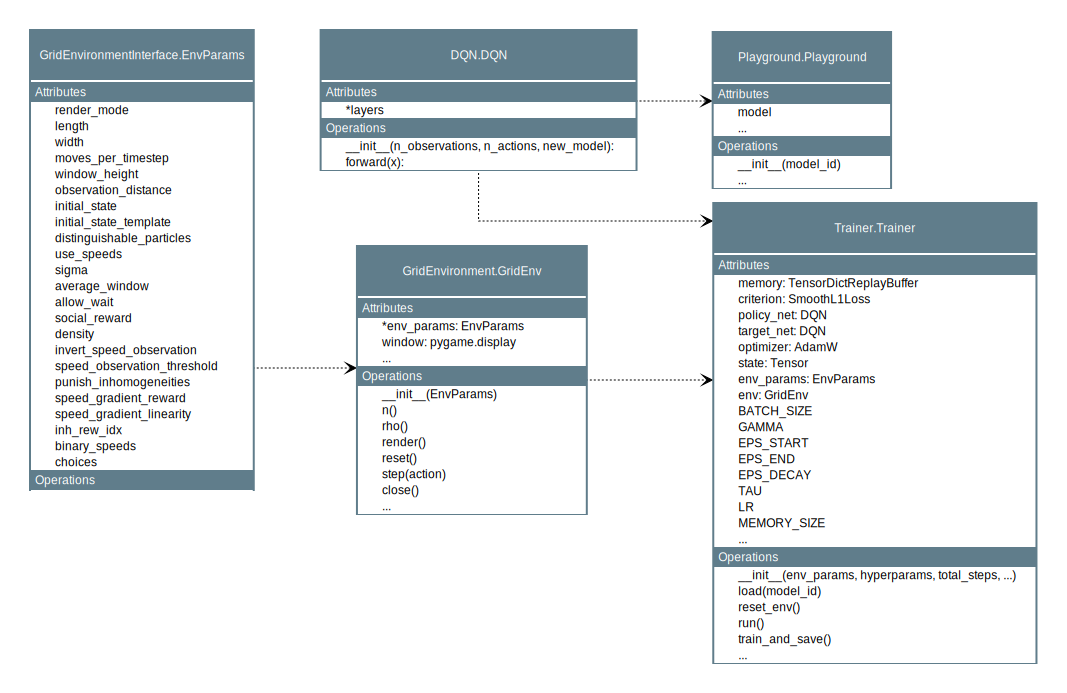
\includegraphics[width=\textwidth]{uml.pdf}
    \caption{UML diagram of the \texttt{SmartTasep} python package. Only selected methods and attributes are shown. The full documentation is available at \cite{maertens_smarttasep_github_2023}.}
    \label{fig:implementation}
\end{figure}


\subsection{GridEnv and EnvParams}
\label{subsec:implementation-gridenv}
The \texttt{GridEnv} class implements the 2D TASEP environment for a reinforcement learning agent. It is a subclass of the \texttt{gym.Env} class from the OpenAI \texttt{gym} library \cite{brockman_openai_2016}. This allows the environment to be used with any reinforcement learning algorithm that is compatible with the OpenAI Gym interface. The environment is initialized with an \texttt{EnvParams} object, which may contain a number of parameters to customize the environment size and initial conditions, the reward structure, the visualization and metrics as well as other properties e.g. to control the dynamics of the reinforcement learning algorithm. 
\\
\\
Internally, the \texttt{GridEnv} class also uses a 2D array to store the state of the system. For indistinguishable particles with equal velocities, this is a binary array, where 0 represents an empty site and 1 represents a site occupied by a particle. Section \ref{subsec:implementation-trainer} will explain that sometimes, particles have to be distinguishable. In that case, the binary array is not suited to store the state. Instead, during initialization, each particle is assigned a unique integer ID, which is stored in the array instead of the ones. If the particles have different velocities, the velocities are stored by adding them to the ID. As the velocities are floats in the range $(0,1)$, they can be stored in the same array without any loss of information. We can retrieve the ID and velocity $v$ of a particle by using the floor and modulo operators on the stored value $s$ respectively:
\begin{equation}
    \text{ID} = \lfloor s \rfloor \text{,} \quad v = s \bmod 1 \text{.}
    \label{eq:state-to-id-velocity}
\end{equation}
This is very memory efficient, as we only need one array to store the state of the system. 
\\
In addition to the state array, the \texttt{GridEnv} also stores the current particle's position in order to be able to calculate the reward after an agent submits its action. 
\\
The following are the two most important methods of the \texttt{GridEnv} class:

\subsubsection{reset}
Resets the environment to its initial state and returns the initial state. Note that in this case, \enquote{state} does not refer to the whole system, but only to the selected particle's observation of the system. 
\\
Agents perceive the system as a $d\times d$ grid centered around them, with the observation distance $d/2$ being a parameter. Observations do not include the particle IDs, as this information is irrelevant to the agent and would even make the problem harder, as the agent would have to learn to distinguish between particles. 
\\
Particle velocities are included in the observations, as they are relevant to the agent. Optionally, the observed velocities can be converted to shifted inverse velocities:
\begin{equation}
    v_{\text{shift, inv}} = 1 - v + v_{\text{shift}} \text{.}
    \label{eq:inverse-velocities}
\end{equation}
This has two possible advantages. Firstly, slow particles are now represented by high values, because they correspond to \enquote{more blockage} in the system. Intuitively, it makes sense to frame the problem in this way, as slow particles are not only worse for the transport, but also more persistent in the observation. Secondly and more importantly, the shift $v_{\text{shift}}$ prevents fast particles from being invisible. Without the velocity inversion, particles with very low velocities become indistinguishable from empty sites, which makes it impossible for the agent to learn to avoid them. The inversion alone does not solve this problem, as particles with very high velocities now become invisible. 
\\
\\
It is important to note that this problem is less about the absolute values of the observations and more about the distinguishability between observations. At first glance, it seems like this rescaling of velocities is not necessary, as the weights can be negative and the biases can be adjusted to compensate for the shifted values. However, this is not the case, as the rescaling is only applied to the particles, not to the empty sites. 


\subsubsection{step}
\label{subsubsec:implementation-step}
Takes an action as an argument and returns the next state and the reward after performing the action. Actions are encoded as integers, which, as we will see, correspond to the index of the output neuron with the highest activation. The form of the next state or states depends on the environment parameters. See section \ref{subsubsec:implementation-train} for more details.
\\
\\
The reward is calculated based on the reward structure that was defined in the \texttt{EnvParams} object. Each option can be included or excluded from the reward calculation, which allows for a high degree of customization. Examples include:
\begin{itemize}
    \item The default structure yields a positive reward for moving forward, a negative reward for trying to move into an occupied site and zero reward for waiting or switching lanes. 
    \item The \texttt{social\_reward} option adds a negative reward switching lanes into a site with a particle behind it. The magnitude of the reward is proportional to the velocity of the blocked particle. The analogy in the traffic flow interpretation is the car horn that a driver behind you would use if you switched lanes in front of them.
    \item The \texttt{punish\_inhomogeneties} option combined with the \texttt{inh\_rew\_idx} parameter can add different complex potential-like rewards to encourage the emergence of global structures. This will be explained in more detail in section TODO
\end{itemize}
When rendering is enabled, the step method also renders the state of the system in regular intervals. The system matrix is rendered using the \texttt{pygame} library, which is fast enough to not bottleneck the simulation. Velocities are encoded as colors using the HSL color space, which makes it easy to convert velocities to hues. The velocity range $(0,1)$ is mapped to the hue range $(0,120)$, which corresponds to the red to green range. 



\subsection{DQN}
\label{subsec:implementation-dqn}
The \texttt{DQN} class implements the deep neural network that is used to approximate the action-values $Q(s,a)$. It is a subclass of the \texttt{torch.nn.Module} class from the PyTorch library. The network has two hidden layers and uses the \texttt{ReLU} activation function introduced in section \ref{subsec:activation-functions}. The output layer uses the identity activation function, as we want to approximate the action-values directly. During initialization, the size of the flattened observation array and the number of actions are passed as arguments, to determine the size of the input and output layers respectively. An additional parameter switches between two 128-neuron hidden layers and a 24-neuron hidden layer followed by a 12-neuron hidden layer. 
\\
\\
As a subclass of the \texttt{torch.nn.Module} class, the \texttt{DQN} class implements the \texttt{forward} method, which performs the forward pass. The \texttt{forward} method can be called with a single observation when evaluating the network or with a batch of observations when training the network. Backpropagation is efficiently implemented in PyTorch using automatic differentiation, as explained in section \ref{subsec:backprop}. During a forward pass, all operations (e.g. network layer operations, activation functions, loss function) automatically store the information that is needed for backpropagation in the \texttt{torch.Tensor} objects used for the calculations. When the \texttt{backward} method is called on the loss tensor at the end of the forward pass, the gradients are automatically calculated and stored in the \texttt{grad} attribute of each tensor. These gradients are then used to update the network parameters as will be explained in section \ref{subsec:implementation-trainer}.



\subsection{ReplayBuffer}
\label{subsec:implementation-replaybuffer}
The replay buffer is also one of the performance-critical parts of the implementation. Instead of a naive custom implementation, the \texttt{SmartTasep} package uses the \texttt{TensorDictReplayBuffer} or \texttt{TensorDictPrioritizedReplayBuffer} classes together with the \texttt{LazyTensorStorage} class from the \texttt{torchrl} library \cite{bou_torchrl_2023}. The \texttt{torchrl} library is a reinforcement learning library based on PyTorch that implements many very efficient modules for high performance reinforcement learning training using parallel environments, multithreading and supports computation on the GPU. The \texttt{ReplayBuffer} classes implement very efficient sampling, storage and priority update of single transitions or batches. 
\\
\\
The \texttt{torchrl} library implements many more features that could be used to improve the performance of the smart TASEP, but due to the limited time of this thesis and the early stage of the library, only the replay buffer was used. The \texttt{SmartTasep} package uses the \texttt{TensorDictReplayBuffer} class for uniform sampling and the \texttt{TensorDictPrioritized\-ReplayBuffer} class for prioritized sampling. The \texttt{LazyTensorStorage} class is used internally by these classes to store the transitions. 



\subsection{Trainer}
\label{subsec:implementation-trainer}
The \texttt{Trainer} class is the heart of the \texttt{SmartTasep} package. It implements the training loop and the evaluation loop as well as some additional functionality such as saving and loading trained agents. The following are the most important methods of the \texttt{Trainer} class:

\subsubsection{Constructor}
The constructor method initializes the \texttt{Trainer} object. It takes a number of parameters:
\begin{itemize}
    \item \texttt{env\_params}: An \texttt{EnvParams} object that contains the parameters for the environment as explained in section \ref{subsec:implementation-gridenv}.
    \item \texttt{hyperparams}: A \texttt{Hyperparams} object that contains the hyperparameters for the reinforcement learning algorithm. The structure of the \texttt{Hyperparams} object is the same as the \texttt{EnvParams} object, but the parameters are different.
    \item Additional keyword arguments that control the training schedule, visualization and general algorithm choices such as the replay buffer implementation or whether different networks should be used for the individual particles.
\end{itemize}
After some basic input validation, e.g. checking if any of the parameter choices are incompatible, the constructor method initializes all subcomponents needed for training and evaluation of the agents as well as the visualization in pygame, the plotting in matplotlib and the accumulation of metrics.
\\
A \texttt{GridEnv} object is initialized with the \texttt{EnvParams} object and \texttt{DQN} objects are initialized as Q-networks and policy networks. Depending on the parameter choices, the Q-network and policy network are either shared between all particles or $n$ pairs of separate networks are initialized. In the latter case, the particle velocity range is divided into $n$ equally sized intervals and each pair of networks is responsible for the particles in one of these intervals. This allows different types of particles (e.g. fast, medium and slow for $n=3$) to learn different policies without the space complexity of a separate network for each particle.
\\
The size of the observation arrays and the action space is determined by the \texttt{GridEnv} object and passed to the \texttt{DQN} objects during initialization. The \texttt{ReplayBuffer} objects are initialized with the corresponding parameters from the \texttt{Hyperparams} object. Furthermore, pytorch's \texttt{SmoothL1Loss} loss function is initialized and pytorch's \texttt{AdamW} optimizers (see section \ref{subsec:sgd}) are initialized for each Q-network. 


\subsubsection{train}
\label{subsubsec:implementation-train}
The \texttt{train} method implements the training loop. As the TASEP is not an episodic task, the method consists of only one loop running the simulation for a specified number of time steps. Optionally, the training can be performed pseudo-episodically, where the environment is reset in regular intervals, possibly with changing initial conditions, for example to train smarticles in environments with variable density. I refer to this as \textit{pseudo}-episodic, as we are still using a replay buffer with stored transitions from previous episodes.
\\
\\
Depending on the parameters, the \texttt{train} method uses slightly different algorithms that differ in the way that transitions are stored in the replay buffer. There are essentially three distinct ways to generate transitions:
\begin{enumerate}
    \item \textbf{Immediate transitions:} The environment returns the observation of the particle that took the action immediately after the action was executed. When this observation is used in transitions, the state-next state pairs contain no information about the environment dynamics, as there is no time between the states for the environment/other particles to react to the action. In this case, the smarticles learn a policy for a static environment, while actually living in a very dynamic environment. Note that in this case, the environment has to also return an additional next state for a new particle in order to move different particles in each time step.
    \item \textbf{Weakly correlated transitions:} This is the natural way to combine algorithms \ref{ch:dql} and \ref{alg:2d-tasep}. The environment returns the next observation after picking a new particle which is then used both as the next state stored in the transition and as the current state for the next action. This method only makes sense when the same networks are shared between all particles, as the next state is not the next state of the particle that took the action. Instead, the network learns a policy for an environment where it is thrown around, each new state seemingly random and only weakly correlated with the previous state. This algorithm is used when the \texttt{distinguishable\_particles} parameter is set to \texttt{False}. TODO: Markovian?
    \item \textbf{Delayed transitions:} When particles are distinguishable and the current particle's ID is returned by the environment together with the next state, the next state in a transition can be set to the observation of the same particle that took the action at the time step where the particle is picked again and has to choose its next action. This generates transitions from the reference frame of the particles. A particle is presented a state (observation) $s$, takes an action $a$ and receives an immediate reward $r$ for that action. It then \enquote{sleeps} until it is picked again and receives a new state $s'$. Between these two observations, the environment has changed, as other particles have moved. The transitions now contain additional information, e.g. that slow particles tend to remain stationary while fast particles tend to move forward. This algorithm is used when the \texttt{distinguishable\_particles} parameter is set to \texttt{True}. It requires a temporary storage of the current state and action for each particle for later use when the particle is picked again. A step by step implementation is provided in pseudocode in algorithm \ref{alg:delayed-transitions}.
\end{enumerate}

\begin{algorithm}[h]
    \caption{DQN with delayed transitions and shared networks (difference to algorithm \ref{alg:dqn} highlighted in \textcolor{red}{red})}
    \label{alg:delayed-transitions}
    \begin{algorithmic}
        \State Initialize replay buffer $\mathcal{D}$ to capacity $N$
        \State Initialize Q-network $Q$ with parameters $\theta$
        \State Initialize target network $\hat{Q}$ with parameters $\theta^-=\theta$
        \State Initialize environment to get initial state $s_1$, \textcolor{red}{initial particle ID $i_1$}
        \State Initialize $\epsilon$ to $\epsilon_0$
        \State \textcolor{red}{Initialize temporary storage $\mathcal{M}$ for $(s,a,r)$ tuples indexed by particle ID}
        \For{steps $t=1,\dots,T$}
            \State $\triangleright$ Generate new transition
            \State Perform forward pass through $Q$ to get action-values $Q(s_t, a')$ 
            \State With probability $\epsilon$ select a random action $a_t$, otherwise select $a_t = \arg\!\max_a Q(s_t, a)$
            \State Execute action $a_t$ in environment and observe reward $r_t$, next state $s_{t+1}$ \textcolor{red}{and ID $i_{t+1}$}
            \color{red}
            \State $\mathcal{M}[i_t] \gets (s_t, a_t, r_t)$ 
            \If{$i_{t+1} \in \mathcal{M}$}
                \State Store transition $(^*\mathcal{M}[i_{t+1}], s_{t+1})$ in $\mathcal{D}$
            \EndIf
            \normalcolor
            \State $\triangleright$ Update Q-network parameters
            \State Sample random minibatch of transitions $(\bm{s}, \bm{a}, \bm{r}, \bm{s'})$ from $\mathcal{D}$
            \State Set $\bm{y} = \bm{r} + \gamma \max_{a'} \hat{Q}(\bm{s'}, a')$
            \State Calculate mean loss $\mathcal{L} = \text{mean}(\mathcal{L}(\bm{y}, Q(\bm{s}, \bm{a})))$
            \State \textcolor{red}{Perform optimization (AdamW) of $\theta$ using backpropagation of $\mathcal{L}$}
            \State $\triangleright$ Update target network parameters
            \State Update target network parameters $\theta^- \gets \tau \theta + (1 - \tau) \theta^-$
            \State $\triangleright$ Update exploration rate
            \State Decrease $\epsilon$   
        \EndFor
    \end{algorithmic}
\end{algorithm}
When different speeds and multiple networks are used, algorithm \ref{alg:delayed-transitions} has to be slightly modified. Instead of $Q$, $\hat{Q}$, $\mathcal{D}$, $\mathcal{L}$ and a single AdamW optimizer for $Q$'s parameters $\theta$, we now have an array of $n$ such objects for each of these modules. The correct objects are chosen in each timestep based on the particle's velocity which is extracted from the state. 

\subsubsection{save and load}
The \texttt{save} method all model parameters and collected metrics logs the ID of the newly saved model. The \texttt{load} method loads the model parameters and metrics of a previously saved model. This allows for easy saving and loading of trained agents. When no ID is provided during loading, a table is shown with all available models and their properties. The user can then select a model to load by entering its ID. The \texttt{train\_and\_save} method provides a wrapper for automatically saving the model after training.

\subsubsection{run}
The \texttt{run} method is a stripped down version of the \texttt{train} method that only runs the simulation for a specified number of time steps, omitting all operations only necessary for parameter optimization. A greedy policy is used instead of the epsilon-greedy policy used during training. This method is used for evaluation of trained agents. 


\subsection{Playground}
\label{subsec:implementation-playground}
The \texttt{Playground} class implements a playground for testing the behavior of trained agents. When run, the user chooses a saved model and is presented with a window of two grids of the same size as the model's observation size. The left grid is empty except for the agent in the middle and can be filled by the user. Clicking a grid cell adds or removes an agent and clicking and dragging adds an agent with a velocity proportional to the drag distance. The right grid shows the same state after the agent has taken an action. Figure \ref{fig:playground} shows a screenshot of the playground.

\begin{figure}[h]
    \centering
    \includegraphics[width=\textwidth]{playground.png}
    \caption{Screenshot of the playground. The state contains one slow particle blocking the agent, a fast particle above the slow one and a particle with average velocity behind the agent. The agent has learned to move around the slow particle in the direction where it's not blocked. More complicated states could be tested e.g. to test the agent's ability to make intelligent decisions based on the speeds and positions of the surrounding particles.}
    \label{fig:playground}
\end{figure}


\section{Hyperparameter Optimization}
\label{sec:hyperparam_optim}
Optimizing the hyperparameters of a reinforcement learning algorithm is a difficult, but important task. Previous research has shown that the choice of hyperparameters can have a significant impact on the performance of the algorithm \cite{henderson_deep_2019,parker-holder_automated_2022,noauthor_automl_nodate}. 
\\
\\
The goal of hyperparameter optimization, or hyperparameter tuning, is to find a set of hyperparameters that maximizes the cumulative reward of the agent. This means that in order to evaluate a set of hyperparameters, we have to train a new agent with these hyperparameters and evaluate its performance by running the simulation for a number of time steps. 
\\
\\
As the choice of one hyperparameter can impact the optimal values of the other hyperparameters, the hyperparameters have to be optimized simultaneously, for example using a grid search or a random search. These algorithms are embarrassingly parallel, as the evaluation of a set of hyperparameters is independent of the evaluation of other sets, but the number of sets that have to be evaluated grows exponentially with the number of hyperparameters. This makes hyperparameter optimization a computationally expensive task.
\\
Due to time constraints, a less computationally expensive approach was chosen for this thesis. Instead of performing a grid search or similar algorithm, the hyperparameters were first roughly optimized by a combination of reference to the literature, intuition and trial and error. Then, starting from this set of hyperparameters, the hyperparameters were optimized one by one, using the best value of a hyperparameter for all further tuning of other hyperparameters. This approach is not guaranteed to find the optimal hyperparameters, but it is computationally cheap and can yield good results. Furthermore, it shows how sensitive the algorithm is to the individual hyperparameters. This knowledge could be used to identify the most important hyperparameters and perform a more thorough optimization of these hyperparameters.
\\
\\
The following eight hyperparameters were optimized:
\begin{itemize}
    \item \textbf{Learning rate} of the AdamW optimizer.
    \item \textbf{Discount factor} $\gamma$.
    \item \textbf{Replay buffer size}.
    \item \textbf{Batch size} for training.
    \item \textbf{Target network update rate} $\tau$.
    \item \textbf{Exploration-exploitation tradeoff} via the decay constant $\eta$ of the exploration rate $\epsilon(t)=\epsilon_{\text{end}} + (\epsilon_{\text{start}} - \epsilon_{\text{end}}) e^{-n_{\text{steps}}/\eta}$.
    \item \textbf{Neural network architecture} (number of hidden layers and neurons per layer).
    \item \textbf{Activation function} of the neural network.
\end{itemize}
It is important to note, that there isn't a single set of hyperparameters that is optimal for deep Q-learning in general. Instead, the optimal hyperparameters depend on the environment and the task. Various studies have shown that reinforcement learning algorithms are very sensitive to the choice of hyperparameters and even the state-of-the-art RL algorithms often fail to generalize beyond their specific task \cite{parker-holder_automated_2022,henderson_deep_2019,engstrom_implementation_2020,andrychowicz_what_2020}. This means that the hyperparameters have to be optimized for each environment and task individually. In this section, we will discuss the hyperparameters that were optimized for the smart TASEP with a simple reward structure that includes only the \texttt{social\_reward} option on top of the default reward (see section \ref{subsubsec:implementation-step}). A relatively high particle density of $\rho=0.5$ was chosen and particle speeds were sampled from a uniform distribution in the range $(0, 1)$.
\\
\\
The starting point for the hyperparameter optimization was the following set of hyperparameters:
\begin{itemize}
    \item \textbf{Learning rate}: $0.005$
    \item \textbf{Discount factor} $\gamma$: $0.8$
    \item \textbf{Replay buffer size}: $10^6$ ($\geq$ number of training steps)
    \item \textbf{Batch size}: $64$
    \item \textbf{Target network update rate} $\tau$: $0.005$
    \item \textbf{Epsilon decay constant}: $10^5$ 
    \item \textbf{Neural network architecture}: 2 hidden layers with 128 neurons each
    \item \textbf{Activation function}: ReLU (output layer uses identity activation)
\end{itemize}
In order to evaluate the performance of the algorithm, the mean reward collected over 10000 time steps was measured in regular intervals of 2500 training steps. For each new hyperparameter value, 100 such episodes of training followed by evaluation were run, training the agents for a total of 250000 optimization steps. The results were plotted with a moving average over 8 and 30 episodes to smooth out the noise. The plots are shown in figure \ref{fig:hyperparam_optim_8} and \ref{fig:hyperparam_optim_30} in appendix \ref{app:hyperparam_optim}.
\\
\\
The following insights were gained from the hyperparameter optimization:
\subsubsection{Epsilon decay}
For this specific reward structure, the exploration-exploitation trade off is not very important. In fact, the experiment suggests that the agent performs slightly better without any exploitation at all. The dense, chaotic environment paired with the random initial weights apparently provides enough exploration to find a good policy even when acting greedily. This is not surprising, as the agent is not required to learn a complex policy, but only to move forward when possible and avoid collisions. A more thorough evaluation of the policies in the playground could provide more insight into the agent's behavior. I expect the reward to be only a rough measure of the agent's \enquote{intelligence}, as it is possible to achieve a high reward by simply waiting for the other particles to move out of the way and moving forward whenever possible. We would expect a more intelligent agent to actively avoid collisions and to treat slow particles differently from fast particles. Examples of such behavior will be analyzed in the next chapter. A decay constant of $10000$ was chosen for the following experiments, as it allows for some exploration in the beginning, but quickly converges to a greedy policy.

\subsubsection{Discount factor}
We see that discount factors in the range $0.5-0.9$ perform best. A slightly smaller discount factor of $0.3$ still performs reasonably well, but a discount factor of $\le0.1$ leads to a significant drop in performance. If the discount factor is chosen too large, the performance seems to oscillate around a lower mean reward. A discount factor of $0.9$ was chosen for the following experiments. Agents trained with this discount factor seem to learn slightly slower than agents trained with a smaller discount factor, but the performance at the end of training is better. I would also expect these agents to learn more complex policies, as they have to take into account the future rewards of their actions. 

\subsubsection{Activation function}
The ReLU and LeakyReLU activation functions perform best, which is not surprising, as they are the most commonly used activation functions in deep learning. The Softsign and tanh functions perform worse and the Sigmoid function performs worst. It is surprising to see that the Sigmoid function performs so much worse than the hyperbolic tangent, as they are rescaled versions of the same function. The tanh should also saturate slightly faster than the Sigmoid function, as it is steeper around the origin. I would expect it to be more prone to vanishing gradients than the Sigmoid function. \\
The ReLU function was chosen in favor of the LeakyReLU function, as it seems to perform equally well and is slightly faster to compute.

\subsubsection{Learning rate}
As expected, large learning rates lead to unstable training and poor performance. They fail to find minima as they keep overshooting, leading to low rewards. Optimal learning rates seem to be smaller than $0.01$ with small variance for values in that range. The optimum seems to be around $0.001$, which is small enough to be stable, but still large enough to allow for fast learning. 

\subsubsection{Batch size}
The batch size seems to be inversely proportional to the speed of convergence of the algorithm. Larger batch sizes converge significantly slower than smaller batch sizes. This can be explained partly by the fact that agents with larger batch sizes start learning later, as they have to collect more transitions before they can collect the first batch and partly by the fact that for smaller batch sizes, the correlation between the transitions in a batch is smaller. Moreover, the scalar loss, which is propagated back through the network, is calculated as the mean loss over the batch. This means that the magnitude of the gradients does not depend on the batch size. The optimum seems to be around $32$. With this batch size, the algorithm converges quickly and reaches the highest mean reward in the end.

\subsubsection{Replay buffer size}
As expected, larger replay buffers perform significantly better than smaller ones. If the buffer is too small, the algorithm fails to converge to a reasonable policy, as not enough independent transitions are stored in the buffer. Larger buffers perform better, saturating of course at the point where the buffer size becomes as large as the total number of transitions that are collected during training. For future experiments, the buffer should be chosen as large as the total number of training steps, if possible. 

\subsubsection{Target network update rate}
The target network update rate seems to have a threshold somewhere between $10^{-5}$ and $10^{-6}$ below which the performance drops significantly. Above this threshold, the performance seems to be only weakly dependent on the update rate, with smaller update rates being more robust. A very large update rate of $0.5$ still produces reasonable results, but the performance oscillates a lot during training. A target network update rate of $0.005$ was chosen for the following experiments, as it seems to be a good compromise between performance and stability.

\subsubsection{Neural network architecture}
In order to test the performance of different neural network architecture, networks with 0-3 hidden layers and different numbers of neurons per layer were trained. A purely linear network with no hidden layers performs very poorly, as expected. Networks with only 6 neurons per layer also perform poorly, although of course much better than the linear network. Interestingly, when only using 6-node hidden layers, the performance seems to decrease with the number of layers. This could be due to the fact that the network is not able to learn a good policy with only 6 neurons per layer, but the additional layers increase the number of parameters that have to be optimized. The best overall performance can be seen for networks with 24 neurons per hidden layer, with more layers performing slightly better than fewer layers. These networks reach almost the same performance as the larger networks by the end of the training, but converge much faster, as fewer parameters have to be optimized. A network with 2 hidden layers and 24 neurons per layer appears to be the best overall choice.

\subsubsection{Summary}
Although a more thorough hyperparameter optimization could be performed, the analysis allows us to gain some meaningful insight into the smart TASEP's sensitivity to different hyperparameters and the ranges of their optimal values. Figure \ref{fig:hyperparam_optim_final_vs_initial} compares the average performance of agents trained with the initial set of hyperparameters and the optimized parameters respectively. We can see that the initial set of hyperparameters was already quite good, achieving convergence to the same mean reward as the optimized set of hyperparameters. However, the optimized set of hyperparameters converges much faster, allowing for an earlier stop of the training.
\\
\\
Note that the acquired set of hyperparameters is only optimal for this specific reward structure. As already mentioned, reinforcement learning algorithms are very sensitive to the choice of hyperparameters and the optimal hyperparameters depend on the environment and the task. In the environment used for this experiment, the conditions stay the same throughout the whole simulation. Imagine for example a reward structure that encourages particle clustering or an environment, where the density is not constant over time. In that case, the epsilon decay constant would probably be an important hyperparameter, as the agent would have to exploit more often in order to generate transitions for the later stages of the simulation. 
\begin{figure}[h]
    \centering
    \includegraphics[width=\textwidth]{hyperparam_optim_initial_vs_final.pdf}
    \caption{Average reward of smart TASEP agents trained with the initial set of hyperparameters and the final set of hyperparameters respectively. The plot is averaged over 10 separate trainings for each set of parameters.}
    \label{fig:hyperparam_optim_final_vs_initial}
\end{figure}

    \graphicspath{{img/results}{img/results/out}}

\chapter{Results}
\label{ch:results}
This chapter will present the results of the smarticle experiments in the TASEP. We will start by setting a baseline with the classical TASEP and analyze how different speed distributions affect this purely stochastic system. Next, we will compare the results with a simple hard-coded policy, before moving on to the smarticle training. We will analyze the results of the smarticle training for different reward structures and compare them to the baseline. 

\section{Notes on measuring time and current}
\label{sec:time_current}
The classical TASEP is defined for continuous time. Each particle moves according to its own internal clock. In the numerical version treated in this thesis, time has to be discretized. The discrete time step should be defined in a way that allows time averages of observables in the discrete version and the continuous version to coincide. We base our time step definition on the fact that in the continuous version, the \textit{average} number of jump attempts per second is constant. We therefore define our time step as a fixed number of \textit{update attempts}. An update attempt is the picking of a random grid cell and the attempt to move the particle in that cell, \textit{if it is occupied}. This means that also in the discrete version, the number of \textit{jump attempts} per second is constant in the time average, while it can fluctuate over short time scales.


In this thesis, the time step is specifically defined as \textit{one} update attempt. This makes it easy to define a particle \textit{current}, which is independent of the system size. The current is defined as the number of actual forward jumps per \textit{update attempt}. This of course has the dimension of a particle current \textit{density}, but it is still called \textit{current} in the lattice gas literature. It is the more useful quantity to work with, as it makes it easy to compare different systems. 


Note that this definition of the time step differs from the prevalent definition of the Monte Carlo time step in the literature \cite[ch. 3.2]{daquila_monte_nodate}, where one time step is defined more naturally as one Monte Carlo sweep. A Monte Carlo sweep is defined as $N$ update attempts, where $N$ is the number of particles in the system. 

\newpage

\section{Setting a Baseline: Classical TASEP}
\label{sec:baseline}
\begin{wrapfigure}{R}{0.45\textwidth}
    \raisebox{0pt}[\dimexpr\height-0.6\baselineskip\relax]{\includegraphics{truncated_normal.pdf}}
    \caption{Normalized truncated normal distributions with mean $\mu=0.5$ and different standard deviations $\sigma$.}
    \label{fig:speed_dists}
\end{wrapfigure}
This section will use the classical 2D (T)ASEP as introduced in section \ref{sec:2d-tasep}. We will make it totally asymmetric in the horizontal direction (the \textit{forward} direction) by setting the probability $p$ to jump forward to $1/2$ and the probability $q$ to jump backward to $0$. The vertical direction (the \textit{up/down} direction) will be symmetric with probabilities $a=b=1/4$. The system has periodic boundary conditions in both directions. We will analyze a $128 \times 32$ system and a narrower $128 \times 6$ system. Both systems will be initialized with a checkerboard pattern of particles and holes, yielding a density of $\rho = 1/2$. This density will be chosen for most experiments, as it is dense enough for the different policies and speed distributions to have a significant effect on the system, but not so dense that the system is always jammed. Speeds will be drawn from a truncated normal distribution with mean $0.5$ and different standard deviations $\sigma$. The distribution is truncated at $0$ and $1$, so that speeds are always in that range. Two example speed distributions are shown in figure \ref{fig:speed_dists}. 

\subsection{Finding the Steady State}

When we want to compare the average current of different ASEP configurations, we have to make sure that the system has reached a steady state. The steady-state has been reached when the current fluctuates around a constant mean value without an overall upwards or downwards trend. The time it takes to reach the steady state depends on the system size, the density and the initial conditions. When using a checkerboard setup for example, it's intuitive that the current will be very high at the beginning of the simulation, as every particle has an empty site in front of it and can move forward. As time passes, the probability of being able to move forward decreases (for different reasons that we will examine in the next paragraphs), and the mean current drops, asymptotically approaching the steady state current.


Figures \ref{fig:currents_fixed_sigma_128x32} and \ref{fig:currents_fixed_sigma_128x3} show the current as a function of time steps since initialization of the system to the checkerboard pattern for different speed distribution standard deviations $\sigma$. We can see that for small $\sigma$, when all particles have similar speeds, the current converges quickly and reaches a steady state after about 100,000-150,000 time steps. For larger $\sigma$, particles have different speeds and the equilibration phase takes longer, as jams form and dissolve and slow particles move very rarely. For $\sigma = 5$, especially in the narrow system (Fig. \ref{fig:currents_fixed_sigma_128x3}), we see that the steady state is still not quite reached after 300,000 time steps. 


One could expect the equilibration time to be roughly proportional to the number of Monte Carlo sweeps that have passed. This, however, is not the case, as we can see by comparing figures \ref{fig:currents_fixed_sigma_128x32} and \ref{fig:currents_fixed_sigma_128x3}. The narrow system has almost 11 times fewer particles than the wide system and thus performs about 11 times more Monte Carlo sweeps in the same number of time steps. However, the equilibration time is not 11 times shorter but seems to be about the same, or even longer. We can conclude that the number of time steps is a better measure of the equilibration time than the number of Monte Carlo sweeps.


For the following experiments, the steady state current will be calculated by running the simulation for 600,000 time steps and averaging the current over the last 150,000 time steps. This ensures that the system has reached a steady state even for the configurations that take longer to equilibrate.

\begin{figure}[H]
    \centering
    \begin{subfigure}{\textwidth}
        \centering
        \includegraphics{currents_fixed_sigma_128x32}
        \caption{System size: 128x32}
        \label{fig:currents_fixed_sigma_128x32}
    \end{subfigure}
    \par\vspace{1cm}
    \begin{subfigure}{\textwidth}
        \centering
        \includegraphics{currents_fixed_sigma_128x3}
        \caption{System size: 128x3}
        \label{fig:currents_fixed_sigma_128x3}
    \end{subfigure}
    \caption{Current as a function of time steps since initialization of the system to the checkerboard pattern for different speed distribution standard deviations $\sigma$ and two different system sizes. The data is averaged over 800 independent runs and plotted with a moving average over 5000 time steps.}
\end{figure}


\section{Steady State Current as a Function of System Size and Speed Distribution}
\label{sec:steady_state_current}
Now that we have established a definition of what is to be measured and how this measurement can be done from the simulation data, we can check if the measured steady state current is in accord with our intuition and how it depends on the system parameters. 

\subsection{Theoretical Expectation}
\label{sec:theoretical_expectations}
In order to derive an expression for the expected value of the current, we closely examine what happens during one time step. This will help us to understand the probability of an actual forward move happening during one time step, which, by our definition, is the current.
\\
The following steps are performed during one time step:
\begin{enumerate}
    \item Pick a random grid cell.
    \item If the cell is occupied (probability $p_{occ}=\rho=0.5$), perform a move attempt as follows:
    \item Check the speed: The move attempt is continued with probability $p_{spd}=\text{speed}$.
    \item If the move attempt is continued, pick a direction (forward has probability $p=1/2$).
    \item If the target cell is empty (probability $p_{emp}\approx 1-\rho$), perform the move.
\end{enumerate}
Where the expression $p_{emp}\approx 1-\rho$ only holds for an approximately uniform density distribution throughout the system. The average speed $\bar{v} = \bar{p}_{spd}$ is the expectation value $\mu$ of the speed distribution, which is set to $0.5$ in all experiments. The total probability of a forward move in one time step is the product of the probabilities of the individual steps:
\begin{align}
    \langle J\rangle &\coloneqq p_{occ} \cdot p_{spd} \cdot p \cdot p_{emp} \label{eq:current_theory} \\
                     &\approx p \cdot \mu \cdot \rho (1-\rho) = \left(\frac{1}{2}\right)^4 \nonumber \\
                     &= 0.0625 \text{.}\nonumber
\end{align}
More thorough derivations of this expression for ASEP systems with equal speeds can be found in the literature, for example in \cite[section 2.3.2]{daquila_monte_nodate}. Equation \ref{eq:current_theory} also confirms that our choice of the density $\rho=1/2$ is optimal for maximizing the current in the system, as the maximum of the function $f(\rho) = \rho(1-\rho)$ is at $\rho=1/2$.


\subsection{Results of the Simulation}
\label{sec:results_simulation_current_sigma_size}
Figure \ref{fig:steady_state_current_sizes_log} shows the steady state current as a function of the speed distribution's standard deviation $\sigma$ for different system sizes. The steady-state current has been obtained as explained previously, and the data is averaged over 800 independent runs. For all system sizes, we observe a constant maximum current for $\sigma \ll 1$ that is only very slightly above the expected value of $0.0625$. The slight increase is probably due to the fact that the steady state is only reached in the limit of infinite time. Although being very close, after 450,000 time steps, the current is still dropping a tiny amount, as can be seen in figure \ref{fig:currents_fixed_sigma_128x3}. 
\\
As the width of the speed distribution grows to values of $\sigma \approx 1$, the current drops quickly before asymptotically converging to the minimum value, following a horizontally inverted logistic function. The logistic curve's midpoint is at $\sigma_0 \approx 0.2$ and the width of the transition is $\Delta \sigma \approx 1$. This makes sense, as the speed distribution is truncated at $0$ and $1$, so for values of $\sigma$ close to $0$, all particles have speeds close to $0.5$ and the current is close to its maximum value. When $\sigma$ grows, the speeds in the system get more and more diverse, until $\sigma$ reaches $1$, where the speed distribution is almost uniform and doesn't change much anymore. 
\\
The current drops although the mean speed in the system is still the same, because the probability of a particle moving forward is not only dependent on its own speed, but also indirectly on the speeds of the particles in front of it. The slow particles bottleneck the current as the fast particles have to wait for them to move forward, creating a jam. This effect is more pronounced in narrower systems, as small jams block a higher proportion of the system. In wide systems, particles can avoid jams by moving around them, and even if there's a jam in almost every lane, the probability of these jams all being in the same column is very low. In narrow systems, this can happen, forming a wall of slow particles, which is hard to penetrate. This is clearly visible in figure \ref{fig:steady_state_current_sizes_log}, where the total drop in current is much higher for narrow systems. 


Looking back at equation \ref{eq:current_theory}, we can also try to explain this behavior theoretically. When jams form, the density in the system is not uniform anymore. Instead, there are regions of high density (jams) and regions of low density (empty lanes). This increases the mean density in the neighborhood of a random particle, decreasing $p_{emp}=(1-\rho)$ and thus the probability of a forward move.  

\begin{figure}[H]
    \centering
    \includegraphics{steady_state_current_sizes_log.pdf}
    \caption{Steady state current as a function of the speed distribution's standard deviation $\sigma$ for different system sizes. Steady-state current is calculated as the average current over all remaining time steps after the steady state has been reached (the current has stopped dropping). The data is averaged over 800 independent runs.}
    \label{fig:steady_state_current_sizes_log}
\end{figure}

\section{A Naive Policy}
We have now established a baseline current for different system sizes and speed distributions. Before we move on to the smarticle training to try to optimize the current with reinforcement learning, let's see if we can improve the current with a simple hard-coded policy. 
\\
One of the simplest and yet effective policies is to always move forward if possible. Especially when we choose $\sigma$ to be very small and all particles have similar speeds, this policy should be very effective, as it keeps the density uniform and avoids jams. Furthermore, it is very easy to implement without writing any new code by just setting the probability $p$ to move forward to $1$ and all other probabilities ($a,b,q$) to $0$.


Figure \ref{fig:steady_state_current_always_forward} compares the steady state current of this policy with the current from the last experiment, again as a function of the width of the truncated normal distribution. We can see that for small $\sigma$, our policy drastically improves the current, approximately doubling it. For larger $\sigma$, the current drops as before and drops even further, resulting in only about half the current of the baseline for $\sigma\gg 1$. 


The reason for the extreme drop in current is that the policy is not able to deal with jams at all. The current in each lane is limited to the speed of the slowest particle in that lane. The resulting measured current then is the average of the currents in all lanes. 

\begin{figure}[H]
    \centering
    \includegraphics{steady_state_current_both_log.pdf}
    \caption{Steady state current as a function of the speed distribution's standard deviation $\sigma$ for two different ASEP configurations. \enquote{Random moves} has a probability of $p=1/2$ to move forward and probabilities $a=b=1/4$ to move up/down. \enquote{Always forward} has $p=1$ and $a=b=0$. A system of size 128x32 was used. The data is averaged over 800 independent runs.}
    \label{fig:steady_state_current_always_forward}
\end{figure}
The current achieved by this policy for small $\sigma$ is even more interesting. It can be used as a new, very strong baseline for smarticle training in systems with equal speeds. At first glance, it might even seem like the theoretical maximum current. Finding this maximum analytically is not trivial and goes beyond the scope of this thesis. However, we can try to find an upper bound for the current by looking at equation \ref{eq:current_theory} again:
\begin{align*}
    \max(\langle J\rangle) &= \max(p_{occ} \cdot p_{spd} \cdot p \cdot p_{emp}) \\
                           &\le \max(p_{occ}) \cdot \max(p_{spd}) \cdot \max(p) \cdot \max(p_{emp}) \\
                           &= \rho \cdot \mu \cdot 1 \cdot \max(p_{emp}) \\
                            &= 0.25 \cdot \max(p_{emp})\text{,}
\end{align*}
where $\max(x)$ is the maximum expected value of $x$ at a random time step, for a randomly picked particle. It therefore represents the maximum time-averaged value of $x$ that can be achieved by any policy. I have set $p_{occ}=\rho$, $p_{spd}=\mu$, as they are external parameters that cannot be optimized by a policy. The policy cannot influence which particle is picked at a given time step, so it cannot influence $p_{occ}$. The \textit{average} speed of a random particle will also always be the mean speed $\mu$. The maximum of $p$ that any policy can have is of course $1$ (in general, this will not be a probability when using a policy, but the decision will be based on the particle's observation, but the maximum fraction of forward decisions is still 1). 
\\
The last factor, $max(p_{emp})$, is the hardest to approximate. There are configurations where $p_{emp}$ reaches its maximum value of $1$, but these configurations cannot last longer than one time step. In the checkerboard configuration, for example, every particle has an empty site in front of it, so $p_{emp}=1$. However, as soon as one particle moves forward, two particles are immediately next to each other, and $p_{emp}$ decreases. We therefore know that $\max(p_{emp})<1$.
\\
On the other hand, we know that $\max(p_{emp})\ge0.5=(1-\rho)$, as this upper bound is reached by the \enquote{always forward} policy. This places the upper bound for the current at
\begin{equation}
    0.25 > \max(\langle J\rangle) \ge 0.25 \cdot (1-\rho) = 0.125 \text{.}
\end{equation}
In order to keep $p_{emp}$ above $1-\rho$, which it would be for a randomized configuration, a policy has to intelligently fight against the disorder inevitably introduced by the random picking of particles. This is especially hard for systems with equal speeds, as the density in these systems has to be kept uniform, while also moving forward as often as possible.
\\
In the regime of high $\sigma$, where the \enquote{always forward} policy performs very poorly, $p_{emp}$ becomes a very interesting point of attack for a current-optimizing policy. When particles have very different speeds, a policy can organize the system in a way that slow particles are more densely packed than fast particles, increasing $p_{emp}$ for the fast particles while decreasing it for the slow particles. This increases the net current, as the fast particles can fulfill their potential to move forward more often. We will investigate this in more detail in the next sections.


\section{Smarticles for Current Optimization}
\label{sec:smarticle_current_optimization}
This section will present the results of different smarticle trainings for slightly different goals. The main goal is always to maximize the current, but we will use different approaches to achieve this goal, utilizing many of the features of the SmartTasep Python package introduced in section \ref{sec:implementation-smarttasep}. Although the deep Q-learning algorithm is not deterministic, e.g. due to the random initialization of the neural network weights, the results presented here have shown to be reproducible. Appendix \ref{app:code} contains the code that is needed to reproduce the results with the SmartTasep Python package.

\subsection{First Training: Equal Speeds}
As a first experiment, we will try to maximize the current in a system with equal speeds. We will use a system of size $128 \times 24$ and a speed distribution with $\sigma=10^{-4}$. The reward structure for this first experiment is very simple and includes only the \texttt{social\_reward} in addition to the default reward. Optimal hyperparameters for this reward structure have already been found in section \ref{sec:hyperparam_optim}. The training was run for 500,000 time steps, with a reset of the environment every 100,000 time steps.


Figure \ref{fig:first_training_screenshot} shows a screenshot of the real-time visualization of the training after $\approx 350,000$ time steps. We can see that the training is almost converged at this point, confirming that $500,000$ time steps are enough to reach convergence for this problem. After the training, the simulation was run with a greedy policy for another $1.5$ million time steps to measure the steady-state current. The results are shown in figure \ref{fig:equal_speeds}. 
\\
We can see that the steady state is reached fairly quickly compared to the stochastic policies. The current fluctuates around a mean value of $0.152$, which is about 143\% higher than the baseline (0.0625) and about 22\% higher than the \enquote{always forward} policy (0.125). The amplitude of the fluctuations is about $0.03$, which is about 20\% of the mean value, but the lowest current measured is still higher than the \enquote{always forward} policy's current. 


These first results are already very promising. One would expect the \enquote{always forward} policy to already perform very well in this simple environment, but the smarticles are able to outperform it by a significant margin. This can be seen as a clear proof of concept, which motivates further experiments with more complex reward structures and speed distributions, as will be presented in the next sections.
\begin{figure}[H]
    \centering
    \includegraphics[width=\textwidth]{first_training_screenshot.png}
    \caption{A screenshot of the real-time visualization of the first training, taken after $\approx 350,000$ time steps. All particles have the same speed of $0.5$, which can also be seen from their yellow color. We can see that the algorithm has almost converged at this point.}
    \label{fig:first_training_screenshot}
\end{figure}

\begin{figure}[H]
    \centering
    \includegraphics{equal_speeds.pdf}
    \caption{Steady state current as a function of the simulation time for the first trained smarticle agent. The green line shows the average current, which is at about $0.152$, outperforming not just the baseline by about 143\%, but also the \enquote{always forward} policy by about 22\%.}
    \label{fig:equal_speeds}
\end{figure}

\subsection{Second Training: Uniformly Distributed Speeds, Simple Reward}
\label{sec:second_training}
We will now move on to a more complex system with almost uniformly distributed speeds ($\sigma=10$). All other parameters are the same as in the first training. A screenshot during the training is shown in figure \ref{fig:second_training_screenshot} and confirms that 500,000 time steps are enough to reach convergence for this problem as well. The new agent was also tested with a greedy policy for another $1.5$ million time steps and the results are shown in figure \ref{fig:uniform_speeds}. This time, more time steps are required to reach the steady state, which makes sense, as the slow particles require more move attempts until they actually move. The mean current is at about $0.117$, again outperforming the baseline ($\approx 0.052$), this time by about 125\%. 


Watching the simulation, we can see that the agent has learned a policy that focuses on the small scale. No large-scale structures like lanes or clusters can be observed. Instead, the global behavior is best described as a meandering flow or a trickle. The slow particles form a quasi-static maze, which the fast particles can navigate through. If the direction of movement was turned from horizontal to vertical, the trickling behavior would look like a Galton board (without the throttle on top and with periodic boundary conditions).

\begin{figure}[h]
    \centering
    \includegraphics[width=\textwidth]{second_training_screenshot.png}
    \caption{A screenshot of the real-time visualization of the second training, taken after $\approx 350,000$ time steps. The particles have different speeds, which can be seen from their different colors. The algorithm has almost converged at this point.}
    \label{fig:second_training_screenshot}
\end{figure}

\begin{figure}[h]
    \centering
    \includegraphics{uniform_speeds.pdf}
    \caption{Steady state current as a function of the simulation time for the smarticle agent trained in an environment with uniformly distributed speeds. The green line shows the average current, which is at about $0.117$, outperforming the baseline by about 125\%.}
    \label{fig:uniform_speeds}
\end{figure}

\subsection{Model Analysis: Explainability}
\label{sec:model_analysis}
We have now seen that the smarticle agent is able to outperform the baseline in two different environments. We also know the algorithm behind the training that is used to find these optimal policies. However, we still don't know \textit{how exactly} the agent is able to achieve this performance. What is the policy that it has learned? What features of the environment are important for the agent? These questions often arise when using deep learning algorithms, as the inner workings of the neural network are not easily accessible, leading some to call deep learning a \enquote{black box} \cite{blazek_blackbox_2022}.


When using machine learning algorithms for real-world applications, especially in direct interaction with humans, it is important to be able to at least partially explain the decisions made by the algorithm. For this reason, a lot of research has been done in the field of \textit{explainable artificial intelligence} \cite{explainable_ai_systematic_2023}. The SHAP (SHapley Additive exPlanations) framework \cite{lundberg_unified_2017, github_shapshap_2024} for example provides a game theoretic approach to explain the output of any machine learning model. It calculates \textit{feature importance} scores, which quantify the impact of each input feature on the model's output. This can provide local explanations for individual predictions as well as global explanations for the model as a whole. Due to the limited time available for this thesis, SHAP or similar feature importance analysis methods have not yet been applied to the smarticles, but this would be an interesting topic for future research.


The smarticles package does, however, provide a simple, \enquote{hands-on} way to analyze the policies: The \texttt{Playground} class, introduced in section \ref{subsec:implementation-playground}, allows us to interactively play with the trained model. This way, we can quickly get a feeling for the policy that the model has learned. This was done for the agent trained with a uniform speed distribution. The results are shown and interpreted in figures \ref{fig:playground_1} to \ref{fig:playground_8}. 

\newcommand\newsubcap[1]{\phantomcaption%
       \caption*{\thefigure\thesubfigure: #1}}

\begin{figure}[H]
        \begin{subfigure}[T]{0.45\textwidth}
            \centering
            \includegraphics[width=\textwidth]{playground/1.png}
            \newsubcap{The agent knows to move forward when there is an empty site in front of it.}
            \label{fig:playground_1}    
        \end{subfigure}
        \hfill
        \begin{subfigure}[T]{0.45\textwidth}
            \centering
            \includegraphics[width=\textwidth]{playground/2.png}
            \newsubcap{The agent knows to move around slow particles.}
            \label{fig:playground_2}
        \end{subfigure}
\end{figure}

\begin{figure}[H]\ContinuedFloat
        \begin{subfigure}[T]{0.45\textwidth}
            \centering
            \includegraphics[width=\textwidth]{playground/3.png}
            \newsubcap{The agent knows which way around a barrier is faster. Right...}
            \label{fig:playground_3}
        \end{subfigure}
        \hfill
        \begin{subfigure}[T]{0.45\textwidth}
            \centering
            \includegraphics[width=\textwidth]{playground/4.png}
            \newsubcap{...or left.}
            \label{fig:playground_4}
        \end{subfigure}
\end{figure}

\begin{figure}[H]\ContinuedFloat
        \begin{subfigure}[T]{0.45\textwidth}
            \centering
            \includegraphics[width=\textwidth]{playground/5.png}
            \newsubcap{The agent knows that fast particles are more likely to move forward than slow particles.}
            \label{fig:playground_5}
        \end{subfigure}
        \hfill
        \begin{subfigure}[T]{0.45\textwidth}
            \centering
            \includegraphics[width=\textwidth]{playground/6.png}
            \newsubcap{The agent knows that sometimes, it's better to wait.}
            \label{fig:playground_6}
        \end{subfigure}
\end{figure}

\begin{figure}[H]\ContinuedFloat
        \begin{subfigure}[T]{0.45\textwidth}
            \centering
            \includegraphics[width=\textwidth]{playground/7.png}
            \newsubcap{The agent tries not to block other particles, if possible.}
            \label{fig:playground_7}
        \end{subfigure}
        \hfill
        \begin{subfigure}[T]{0.45\textwidth}
            \centering
            \includegraphics[width=\textwidth]{playground/8.png}
            \newsubcap{If the agent has to block other particles, it tries to block slow particles.}
            \label{fig:playground_8}
        \end{subfigure}
\end{figure}

We can see that the agent has learned a complex policy, that not only enables it to navigate around obstacles but also takes into account the speed of the other particles that make up the obstacle. In all eight situations that were tested, the agent made the logical decision, which is also the decision that a human would make in the same situation, and it has also learned to incorporate some social behavior into its policy. A possible next step for further research on an application of the smarticles could be to dive deeper into the basic rules by which the agent makes its decisions, also quantifying the confidence of the agent in its decision. That knowledge could then be used to fine-tune the policy in areas where it is not yet optimal, to provide explainability, and also to strip down the policy to a less complex, but still effective version, that uses less computational resources and is faster to evaluate. 

\section{Encouraging Global Structures}
\label{sec:global_structures}
We have already seen two different policies that both perform very well, but until now, the smarticles have only learned to act on their own, although some social behavior is incorporated into the previous policies. It could, however, be beneficial to encourage the formation of global structures, like lanes or clusters. 


For one, this could improve the total current, as a higher priority could be assigned to the fast particles, allowing them to move in a lower-density environment, while the slow particles are more densely packed. Even with uniform density throughout the system, the formation of \textit{fast lanes} and \textit{slow lanes} could be beneficial, as it prevents the fast particles from getting stuck behind slow particles.
\\
Furthermore, even outside the context of current optimization, global structures are important for the stability of the system. When the system is not periodic in the transverse direction, the particles have to be kept together to efficiently create a directed flow. Imagine a real-world application where smarticles are not moving on a tube's surface but on a plane. In this case, the width of the particle stream would increase with the distance traveled. This is because although the mean movement in the transverse direction is zero, the variance is not. For such a system, it is important to keep the particles together, which can be achieved by encouraging the formation of global structures.

\subsection{A Physicist's Perspective on the Reward Structure}
\label{sec:physics_reward_structure}
The formation of global structures arising from microscopic interactions is an interesting point to again make the connection to physics. We can compare the way physical matter is formed from physical particles with the way that smart matter is formed from smarticles. 


Physical matter in thermodynamic equilibrium organizes in a way that minimizes or maximizes a certain thermodynamic potential such as the free energy or the entropy. This is the result of the microscopic interactions between the particles that make up the matter. For most systems, it is not feasible to describe the microscopic state of a system as a function of time, as the number of degrees of freedom grows exponentially with the number of particles. Instead, we use statistical mechanics to describe the system in terms of macroscopic observables, such as the density or the temperature. We can then derive the expected value of these observables by averaging over all possible microscopic states of the system.


Similarly, when using reinforcement learning to train a system of smarticles, we try to define a high-level quantity that we want to optimize, such as the current. We then use this quantity as a reward signal to train the smarticles to maximize it. The microscopic interactions between the smarticles are learned and therefore \textit{defined} by the smarticles themselves, without us having to worry about them. In a sense, we let the smarticles discover the \enquote{physical} laws that would have to govern the system in order to maximize the reward. As a next step, we can then try to derive these laws from the trained policy, as we have done in section \ref{sec:model_analysis}.


Sometimes, different laws (policies) can lead to very different macroscopic behavior while still maximizing the same high-level quantity. For example, the current can be maximized by a policy that keeps the system mixed, as well as by a policy that forms lanes (different local minima that the gradient descent algorithm can converge to). One could compare this to the different phases of matter in physics, where the laws that govern the microscopic interactions are the same, but the macroscopic behavior changes drastically, often also involving symmetry breaking. Here, however, the laws are different, while the high-level quantity that is optimized is the same. The macroscopic behavior arising from the new laws of interaction may still be very similar to the behavior arising from the old laws, but it could also be very different. 


When trying to encourage the formation of global structures, we are trying to nudge the smarticles towards a certain set of laws that we think will lead to the desired behavior, \textit{while still maximizing the current} (In machine learning language, we're helping the gradient descent algorithm to find a specific local minimum, instead of a random one closest to the initial conditions. Alternatively, one could understand it as a way of actively enforcing exploration \textit{in the right direction}).  We do this by incorporating a new reward signal into the reward structure, which is based on the microscopic state of the system. In order to find a suitable reward signal, we \textit{can} look back at physics, drawing inspiration from the laws that govern the formation of global structures in physical equilibrium matter.

\subsection{Global Structures - The Easy Way}
\label{subsec:global_structure_easy}
The first approach that we will try is to very explicitly supply the smarticles with the structure that we want to see. This can be done by supplying the agents with their absolute position on the transverse axis (with to an arbitrary origin) as an additional input feature. We can then create a reward function that is based on this position as well as the speed of the particle. The \texttt{speed\_gradient\_reward} function in the smarticles package implements this idea. It assigns a desired lane to the particle based on its speed and then rewards the agent proportionally to the distance to that lane. The speeds are mapped to lanes using the following function:
\begin{equation}
    \Delta y=1-a\cdot\left(\frac{\left(1+a\right)}{a}\right)^{v}+a \text{,}
\end{equation}
where $\Delta y$ is the relative distance from the center ($\Delta y=1$ is a distance of \texttt{system width / 2} from the center) and $v$ is the speed of the particle. The parameter $a$ controls the steepness of the function. In the limit of $a\rightarrow\infty$, the function becomes linear with a slope of $1$, while for small $a$, the function grows exponentially. This allows us to assign a higher proportion of lanes to the fast particles. Figure \ref{fig:speed_gradient} shows the mapping for different values of $a$. The decision to put the center lane into the middle of the screen is of course arbitrary, as the system is periodic in the transverse direction. 
\begin{figure}[H]
\centering
\begin{subfigure}{\textwidth}
    \centering
    \includegraphics[width=\textwidth]{speed_gradient_0.4}
\end{subfigure}
\begin{subfigure}{\textwidth}
    \centering
    \includegraphics[width=\textwidth]{speed_gradient_100}
\end{subfigure}
\caption{The mapping of speeds to lanes in the \texttt{speed-gradient-reward} function for different values of $a$. The images left of the graph are screenshots of the real-time visualization of the simulation.}
\label{fig:speed_gradient}
\end{figure}
Figure \ref{fig:speed_gradient} also shows screenshots of the simulation after training. We can see that the formation of lanes clearly works, and the actual color gradient realized by the smarticles in the system closely matches the desired gradient which is encoded in the reward. In the screenshot corresponding to a non-linear mapping ($a=0.4$), we can see that the mean density in the fast lanes is indeed lower than in the slow lanes. We will investigate the effect that this has on the current in a minute. 


The two screenshots also include examples of imperfect behavior. For one, we always see stray slow particles in the fast lanes, as it takes them a long time to move to their desired lanes. This is something that resolves itself over time, but it also doesn't decrease the current too much, as long as the slow particles don't happen to be oriented in a vertical line. 
\\
The second problem that can arise is visible in the screenshot of the linear gradient system ($a=100$). Here, we can see that the fast particles seem to form clusters also in the horizontal direction, which is not desired. This problem can be fixed by adjusting the ratio of the magnitude of the clustering reward to the magnitude of the default \textit{forwards} reward. If the forward reward is low compared to the clustering reward, the agent will focus more on clustering than on moving forward. This is something one has to always keep in mind when combining different reward signals together.


Next, we will analyze the effect of the \texttt{speed\_gradient\_reward} on the current. We will pick the system with $a=0.4$ as it is the most interesting one, actually prioritizing the fast particles over the slow particles. As the equilibration time for this policy is longer than for the previous policies, the simulation was run for 8.5 million time steps. The results are shown in figure \ref{fig:speed_grad_current}. 


We can see that the current shows a steep increase in the beginning, while the slower particles are still moving to their desired lanes. The slope then decreases as the slowest particles try to reach their lanes and eventually converges to a steady state value of about $0.134$. This is about 15\% higher than the current of the previous policy and about 157\% higher than the baseline. The whole equilibration process can be seen as a video at \cite{maertens_smarticle_lane_vid}.

\begin{figure}[H]
    \centering
    \includegraphics{speed_grad_current.pdf}
    \caption{Current as a function of the simulation time for the smarticle agent trained with the \texttt{speed\_gradient\_reward} function with $a=0.4$ and an almost uniform speed distribution with width $\sigma=5$. The green line shows the average current during the last 1.5 million time steps of the simulation, which is at about $0.134$, outperforming the last policy by about 15\% and the baseline by about 157\%.}
    \label{fig:speed_grad_current}
\end{figure}

After these results, it is clear that even if the lane strategy may not be \textit{the} most efficient transport strategy for the TASEP, it still clearly outperforms the meandering flow strategy and is, therefore, a very promising approach. The next step will be to try to encourage the formation of lanes in a more natural way, without explicitly supplying the smarticles with the desired structure.
\\
The current approach for lane formation is not easy to implement in a real-world application, as it requires the smarticles to communicate in order to agree on a common origin. One could of course also think about the smarticles moving in an external potential, but this could hardly be called a \textit{physical} potential. It would have to be a trapping potential in one direction while allowing movement in the other direction and most importantly, the minimum of the potential (the location of the trap) would have to be different for different speeds. Research on such potentials has been done in the context of trapped ion quantum computers, giving rise for example to the Paul trap \cite[II.A]{bruzewicz_trapped-ion_2019}. It would, however, be easier if the smarticles could form lanes just by local interactions. This is what we will try to achieve in the next section.

\subsection{Global Structures - The Nice Way}
\label{subsec:global_structure_nice}
In this second structure-emergence experiment, we will try to let global structures emerge just from local \enquote{interactions}. Local interactions, in this context, are again the physical analogy to what we're really doing: Finding a reward function that is just based on the observation of a single particle. This, however, is a much harder endeavor than the previous approach. We will therefore introduce two modifications to the experiment:
\begin{enumerate}
    \item We will limit the speed distribution to a binary distribution with only two speeds: $0.25$ and $0.95$. This will make it easier for the smarticles to form lanes, as it reduces the complexity of the problem. Instead of a quasi-continuous gradient, the smarticles now only have to form two distinct lanes.
    \item We will use two different neural networks (pairs of networks) for the two types of particles as explained in \ref{subsubsec:implementation-train}. Although the network was already supplied with the speed of the current particle as an input feature, it is still much easier this way. When two types of particles have to behave differently, it means that the same input vector has to be mapped to an entirely different output vector in some situations, just based on the speed of the particle. To facilitate this, we would want the network weights to depend on the speed of the current particle, which is what we achieve by using two different networks. Furthermore, the performance of the simulation is hardly affected by this change, as only one of the networks has to be used at any given time step. Training does, however, take twice as long, as each network only receives half the training data (only the transitions of the particles with the corresponding speed).
\end{enumerate}
The hardest part of this experiment is to find a suitable reward function. I will just present a working reward function here before we proceed to analyze it. The reward function that is used in the smarticles package to achieve the emergence of lanes is defined as follows:
\begin{equation}
    \text{V}(r, \Delta v) = \begin{cases}
        -0.125 \cdot r + 0.625 & \text{if } \Delta v < 0.5 \text{ and } 1.5 < r \le 5 \\
        -0.75 \cdot r^{-1.3} - 0.15 & \text{if } \Delta v \ge 0.5 \text{ and } r \le 3.5 \\
        0 & \text{otherwise} \text{,}
    \end{cases}
    \label{eq:lane_reward_func}
\end{equation}
where $r$ is the distance between two particles and $\Delta v$ is the difference in speed between them. This pairwise potential is taken between the current particle and every other particle in its observation and summed up to form the reward. 


This might look complicated at first, but it will make sense after analyzing its basic properties. Let's turn to figure \ref{fig:lane_reward_func_3d} to get a better understanding of the reward function. We start by looking at the portion of the potential for $\Delta v > 0.5$ (the front left part of the plot). Here, the potential is less than or equal to zero for all distances. For distances larger than $r=3.5$, the potential is zero. For smaller distances, the potential is negative and decreases with decreasing distance. This just means that the agent is punished (negative reward) for being close to particles that have a very different speed ($\Delta v > 0.5$). This part tries to separate the fast and slow particles, but it isn't enough to form lanes already. Imagine a crowd of two kinds of people, homogeneously mixed. If everyone just tries to keep their distance from people of the other kind, the result will still be a mixed crowd with no structure.
\\
This is where the posterior portion of the potential comes into play. For $\Delta v < 0.5$, the potential is positive and increases with decreasing distance. This means that the agent is rewarded for being close to particles with a similar speed. For distances smaller than $r=1.5$, the potential drops back to zero, so as to keep the density inside the lanes low enough to move.


The combination of these two potentials is what makes the lanes emerge. The particles are rewarded for clustering together with particles of similar speed and these clusters are then separated by the negative reward between particles of different speeds. If the reward for forward moves is high enough compared to the clustering reward, the clusters will naturally stretch out in the forward direction, forming lanes. Alternatively, one could also try to let the potential depend only on the vertical distance between the particles to dampen the effect of the potential on the horizontal movement. 

\begin{figure}[H]
    \centering
    \includegraphics{lane_reward_func_3d_cropped.pdf}
    \caption{The reward function (\enquote{potential}) that achieves the emergence of large fast and slow lanes in the system. It takes the velocity difference and the distance between two particles as input. The potential is calculated between the agent and every other particle in the current observation and then summed up.}
    \label{fig:lane_reward_func_3d}
\end{figure}

After calling this function \enquote{potential} for the last few paragraphs, let's quickly look at why this makes sense. A physical potential gives rise to a force (its gradient) that drives the particles toward a configuration of (locally) minimal energy. In our case, the total reward takes the role of the energy and the algorithm tries to \textit{maximize} it. This is why contrary to physics, the negative areas of our potential are repulsive, while the positive areas are attractive. The \enquote{forces} in our case are encoded into the learned policy of the smarticles. In the general case of a partly stochastic policy, one could call these forces \enquote{voluntary forces}, as an agent doesn't necessarily follow the force that is applied to it. Another important distinction is that when the discount factor is large enough, the agent will value the future reward higher than the immediate reward. This can lead to a policy that actually moves \textit{away} from a local maximum of the reward if it can reach a higher maximum in the future. This is something that fundamentally distinguishes smart matter from physical matter, as physical matter will always move towards a local minimum of the potential, possibly getting stuck in a local minimum that is not the global minimum. (Note that this \textit{can} of course also happen in smart matter)


The proposed reward structure was put to the test in different trainings and subsequent simulations. Training an agent with a complicated reward function makes the training process less stable, and the final policies may differ. Depending on which exact realization of the lanes is discovered first, policies can have a slight bias towards a lane tilt in either direction or a suboptimal tendency to cluster also in the horizontal direction, leading to jams. I will present different approaches to mitigate these problems in the future, after the analysis of the current performance. Figure \ref{fig:lanes} shows two screenshots of different trained agents. While the policy in figure \ref{fig:lanes_straight} has learned to form straight, horizontal lanes, the policy in figure \ref{fig:lanes_tilt} has a slight bias towards going up, leading to a tilted lane structure. Furthermore, both screenshots show a two- to three-cell gap between the lanes. This is suboptimal, as the unused space could be filled with particles, lowering the mean density in the lanes and therefore increasing the current. 

\begin{figure}[H]
    \centering
    \begin{subfigure}{\textwidth}
        \centering
        \includegraphics[width=\textwidth]{lanes_straight.png}
        \caption{These agents have learned to form straight lanes}
        \label{fig:lanes_straight}
    \end{subfigure}
    \vskip\baselineskip
    \begin{subfigure}{\textwidth}
        \centering
        \includegraphics[width=\textwidth]{lanes_tilt.png}
        \caption{These agents have learned a small bias towards going up, leading to a tilted lane structure}
        \label{fig:lanes_tilt}
    \end{subfigure}
    \caption{Screenshots of the real-time visualizations of the simulation for two different policies trained with the \texttt{lane\_reward} function. The agents have learned to form lanes, but the lanes are not always perfectly straight. The environment has a density of $\rho=0.4$ and a binary speed distribution with speeds $0.25$ and $0.95$.}
    \label{fig:lanes}
\end{figure}

\begin{figure}[h]
    \centering
    \includegraphics{lanes_current.pdf}
    \caption{Current as a function of the simulation time for the smarticle agent trained with the \texttt{lane\_reward} function. The green line shows the average current, which is at about $0.112$. The current is consistently higher than the baseline but lower than that of the previous policies.}
    \label{fig:lanes_current}
\end{figure}

For one of the lane-forming agents, the current was again measured over time. The results are shown in figure \ref{fig:lanes_current}. The current fluctuates around a mean value of about $0.112$. We don't have a baseline for this configuration yet, as the density has been changed to $\rho=0.4$ to make the organization easier, and the mean speed is now $0.6$, which is higher than the speed of the baseline. We can set an optimistic baseline using equation \ref{eq:current_theory}, yielding $J_{\text{baseline}}=0.4\cdot(1-0.4)\cdot0.6\cdot0.5=0.072$. The current of the lane-forming policy would then be about 56\% higher than the baseline, but a lot lower than the current of the previous policies. The magnitude of the fluctuations is about $0.02$, about as large as that of the meandering flow policy. The speed gradient policy has a much smaller fluctuation amplitude, as the \enquote{hard coded} structure of the lanes is much more stable than the emergent structure. The equilibration time of the lane-forming policy is very short compared to the last policy, partly because the lower density and the lack of very slow particles make it easier for the particles to move to their desired lanes, and partly because the center is not fixed to a specific lane, but can arise naturally from the initial conditions. A video of the simulation can be found at \cite{maertens_smarticle_lane_vid_local}.


Compared to the previous sections, these results may seem underwhelming at first. This experiment does, however, serve as a proof of concept, showing that it is possible to encourage the formation of global structures in the smarticles from local interactions. Combined with the results of the previous section, we can conclude that the lane-forming strategy is a very promising approach for smarticle applications in transport optimization. The following points can be identified as possible next steps to improve and build on the potential defined in equation \ref{eq:lane_reward_func}:
\begin{itemize}
    \item \textbf{Different Speeds:} The current experiment was done with a binary speed distribution. It would be interesting to see if the same strategy can be applied to a more complex speed distribution, starting with discrete distributions with more than two speeds and then moving on to continuous distributions, possibly binning the speeds into discrete intervals that are mapped to different networks. 
    \item \textbf{Asymmetry:} The absolute value of particle speeds could be incorporated into the attractive part of the potential so that particles with lower speeds cluster closer together than particles with higher speeds. The same has proven to be beneficial for the speed gradient policy, increasing the current.
    \item \textbf{Efficiency:} One of the main problems of the current policy is the gap between the lanes. This could potentially be fixed by restricting the repulsion between particles of different speeds to a smaller range, so that slow particles are pushed out of the fast lanes, but not further away from them (and vice versa). One could also try to include a very short-range repulsion between particles of the same speed, to prevent them from clustering too closely together. This already happens to some extent, as particles are rewarded more for being further than $r=1.5$ away from particles of the same speed, than for being closer than that. The height of this step in the potental could be increased. 
\end{itemize}

\chapter{Conclusion and Outlook}
\label{chap:conclusion}
The goal of this thesis was to investigate the potential of smart matter as a tool for transport optimization in systems that obey the rules of the simple exclusion process. We have explored the foundations of machine learning, especially reinforcement learning with deep neural networks, and have seen how these algorithms can be combined with the simple exclusion process in two dimensions to create a simulation of smarticles. This theoretical framework was implemented in the modular \texttt{smarttasep} Python package, which was eventually used to train and test different smarticle agents.


After establishing a baseline with the classical stochastic TASEP model as well as a simple, hard-coded policy, we showed that a very simple reward structure is enough for a smarticle agent to learn a policy that not only massively outperforms the baseline, but also includes some simple social behavior. A hands-on analysis of the policy on the \texttt{Playground} has proved to be a very useful tool to get an intuitive understanding of the policy that the agent has learned.


We realized that simple rewards will in general only lead to the convergence of the DQN algorithm to a local extremum, and in our case to a simple, yet effective policy. In order to investigate the potential of more complex policies, we have introduced a reward structure that encourages the formation of global structures, to try to nudge the algorithm towards a more complex policy that potentially increases the current even more. The search for these lane-forming policies was successful, resulting in two proof-of-concept policies. 
\\
The first one uses a very explicit reward structure that is based on the absolute position of the particle on the transverse axis. Although this approach is not very practical for most real-world applications, it has shown that the formation of lanes is a very promising approach to increasing the current. 
\\
The second approach uses a more natural reward structure that is based on the observation of a single particle. The version presented in this thesis was not able to outperform the simple policy, but it showed that lane structures can emerge from local interactions. It can serve not just as a proof of concept but also as a building block for future research. Different proposals for improvements and next steps have been presented. 


I think that the final results, for one, show that the smarticles are a very promising tool for transport optimization in suitable systems and could be used for various real-world applications such as traffic optimization for self-driving cars or the directed transport of medicine in the human body by smart nanobots. 
\\
For another, this thesis was an interesting dive into the world of machine learning and smart matter. Both fields are very active areas of research, and I'm sure that we will see a lot of exciting developments in the future. Along the way, we have stopped several times to make connections to physics and to pinpoint the fundamental differences between smart matter and physical equilibrium matter. I think that this is a very interesting topic, as it shows that smart matter is not just a tool, but also a very interesting research topic in itself. I hope that this thesis can serve as one of the early examples of smart matter simulations and that the modular \texttt{smarttasep} package could be used as a building block for future research on similar topics. 


    \newpage
    \thispagestyle{plain}

    \begin{appendix}
        \graphicspath{{img/appendix}{img/impl}}

\newcommand\invisiblesection[1]{%
  \refstepcounter{chapter}%
  \addcontentsline{toc}{chapter}{\protect\numberline{\thechapter}#1}%
  \sectionmark{#1}}

\invisiblesection{Hyperparameter Optimization}
\subsubsection{Hyperparameter Optimization Plots (moving avg. of 8)}
\label{app:hyperparam_optim}
\begin{figure}[H]
    \advance\leftskip-2.3cm
    \includegraphics[width=1.28\textwidth]{hyperparam_optim_8_sci.pdf}
    \caption{Hyperparameter optimization plots analyzed in section \ref{sec:hyperparam_optim}.}
    \label{fig:hyperparam_optim_8}
\end{figure}

\subsubsection{Hyperparameter Optimization Plots (moving avg. of 30)}
\label{app:hyperparam_optim_30}
\begin{figure}[H]
    \advance\leftskip-2.3cm
    \includegraphics[width=1.28\textwidth]{hyperparam_optim_30_sci.pdf}
    \caption{Hyperparameter optimization plots analyzed in section \ref{sec:hyperparam_optim}.}
    \label{fig:hyperparam_optim_30}
\end{figure}


\chapter{Code}
\label{app:code}

This appendix contains the code that is needed to reproduce the results presented in this thesis. The code depends on the \texttt{smarttasep} package, which can be installed on your system (or in a virtual environment) after setting up the python interpreter by running 
\begin{minted}
    [bgcolor=LightGray, fontsize=\footnotesize]
    {bash}
  python -m pip install smarttasep
\end{minted}
On some systems, the \texttt{python} command might be replaced by \texttt{python3} or \texttt{py}. The library's source code can be found at \cite{maertens_smarttasep_github_2023}.
\\
\\
Only the code for running the training is shown here. After training, the model is automatically saved and the unique model ID is printed to the console. Models can be evaluated by running the simulation:
\begin{minted}
    [bgcolor=LightGray, fontsize=\footnotesize]
    {python}
from smarttasep import Trainer

trainer = Trainer.load(model_id=1, total_steps=1_500_000)

trainer.run(reset_stats=True)
\end{minted}
or by launching the \texttt{Playground}:
\begin{minted}
    [bgcolor=LightGray, fontsize=\footnotesize]
    {python}
from smarttasep import Playground

Playground(model_id=1)

\end{minted}


\section{First training: Equal Speeds}
\label{app:first_training}
\begin{minted}
    [bgcolor=LightGray, fontsize=\footnotesize, linenos, breaklines]
    {python}
  from smarttasep import Trainer, Hyperparams, EnvParams

  if __name__ == '__main__':
      envParams = EnvParams(render_mode="human",
                            length=128,
                            width=24,
                            moves_per_timestep=200,
                            window_height=200,
                            observation_distance=3,
                            distinguishable_particles=True,
                            initial_state_template="checkerboard",
                            social_reward=True,
                            use_speeds=True,
                            sigma=0.0001,
                            allow_wait=True,
                            invert_speed_observation=True,
                            speed_observation_threshold=0.35)

      hyperparams = Hyperparams(BATCH_SIZE=32,
                                GAMMA=0.85,
                                EPS_START=0.9,
                                EPS_END=0.05,
                                EPS_DECAY=100_000,
                                TAU=0.005,
                                LR=0.001,
                                MEMORY_SIZE=500_000)
  
      trainer = Trainer(envParams, hyperparams, reset_interval=100_000,
                        total_steps=500_000, do_plot=True, plot_interval=4000, new_model=True)
  
      trainer.train_and_save()
\end{minted}

\section{Second training: Uniformly Distributed Speeds, Simple Reward}
\label{app:second_training}
\begin{minted}
    [bgcolor=LightGray, fontsize=\footnotesize, linenos, breaklines]
    {python}
from smarttasep import Trainer, Hyperparams, EnvParams

if __name__ == '__main__':
    envParams = EnvParams(render_mode="human",
                          length=128,
                          width=24,
                          moves_per_timestep=200,
                          window_height=200,
                          observation_distance=3,
                          distinguishable_particles=True,
                          initial_state_template="checkerboard",
                          social_reward=True,
                          use_speeds=True,
                          sigma=10,
                          allow_wait=True,
                          invert_speed_observation=True,
                          speed_observation_threshold=0.35)

    hyperparams = Hyperparams(BATCH_SIZE=32,
                              GAMMA=0.85,
                              EPS_START=0.9,
                              EPS_END=0.05,
                              EPS_DECAY=100_000,
                              TAU=0.005,
                              LR=0.001,
                              MEMORY_SIZE=500_000)

    trainer = Trainer(envParams, hyperparams, reset_interval=100_000,
                      total_steps=500_000, do_plot=True, plot_interval=4000, new_model=True)

    trainer.train_and_save()
\end{minted}


\section{Global Structures - The Easy Way}
Edit the \texttt{speed\_gradient\_linearity} parameter as needed.
\begin{minted}
    [bgcolor=LightGray, fontsize=\footnotesize, linenos, breaklines]
    {python}
from smarttasep import Trainer, Hyperparams, EnvParams

if __name__ == '__main__':
    envParams = EnvParams(render_mode="human",
                          length=128,
                          width=32,
                          moves_per_timestep=80,
                          window_height=300,
                          observation_distance=3,
                          distinguishable_particles=True,
                          initial_state_template="checkerboard",
                          social_reward=False,
                          use_speeds=True,
                          sigma=5,
                          allow_wait=True,
                          invert_speed_observation=True,
                          speed_observation_threshold=0.35,
                          punish_inhomogeneities=False,
                          speed_gradient_reward=True,
                          average_window=2000,
                          speed_gradient_linearity=100)

    hyperparams = Hyperparams(BATCH_SIZE=128,
                              GAMMA=0.99,
                              EPS_START=0.9,
                              EPS_END=0.05,
                              EPS_DECAY=50_000,
                              TAU=0.005,
                              LR=0.005,
                              MEMORY_SIZE=900_000)

    trainer = Trainer(envParams, hyperparams, total_steps=900_000, new_model=false)

    trainer.train_and_save()
\end{minted}

\section{Global Structures - The Nice Way}
\begin{minted}
    [bgcolor=LightGray, fontsize=\footnotesize, linenos, breaklines]
    {python}
from smarttasep import Trainer, Hyperparams, EnvParams

if __name__ == '__main__':
    envParams = EnvParams(render_mode="human",
                          length=100,
                          width=10,
                          moves_per_timestep=200,
                          window_height=100,
                          observation_distance=4,
                          distinguishable_particles=True,
                          density=0.4,
                          use_speeds=True,
                          sigma=5,
                          allow_wait=false,
                          invert_speed_observation=True,
                          speed_observation_threshold=0.35,
                          punish_inhomogeneities=True,
                          inh_rew_idx=0,
                          speed_gradient_reward=False,
                          average_window=4000,
                          binary_speed=True)

    hyperparams = Hyperparams(BATCH_SIZE=64,
                              GAMMA=0.8,
                              EPS_START=0.9,
                              EPS_END=0.05,
                              EPS_DECAY=150_000,
                              TAU=0.005,
                              LR=0.005,
                              MEMORY_SIZE=500_000)

    trainer = Trainer(envParams, hyperparams, total_steps=1_500_000, new_model=True, random_density=False, diff_models=True, num_models=2)

    trainer.train_and_save()
\end{minted}
        \chapter*{Acknowledgements}\label{chap:acknowledgements}
\lipsum[1]
    \end{appendix}

    \newpage
    \thispagestyle{empty}
    \addcontentsline{toc}{chapter}{References}
    \printbibliography


    \clearpage{\pagestyle{empty}\cleardoublepage}
    \thispagestyle{empty}
\vspace*{1cm}
{\huge \textbf{Selbständigkeitserklärung}}\\
\vspace*{1.5cm}

Ich versichere hiermit, die vorliegende Arbeit mit dem Titel

\begin{center}
    \textbf{Titel der Arbeit}
\end{center}

selbständig verfasst zu haben und keine anderen als die angegebenen Quellen und Hilfsmittel verwendet zu haben.
\\
Die Nutzung von Tools, die auf generativer künsticher Intelligenz basieren, geht nicht über Rechtschreib- und Grammatikprüfung sowie Formulierungshilfen hinaus.

\vspace*{3cm}

Jonas Märtens

\vspace*{1cm}
München, den 15.~Januar 2024

\end{document}